\appchapter{CUDA-multi Experiments}
\label{appendix:experiments:cudamulti}
% SECTION START %
\section{Version Experiments (Best Runtimes)}
\begin{figure}[H]
\begin{adjustwidth}{-2cm}{-2cm}
\centering
\begin{subfigure}{.62\textwidth}
    \centering
    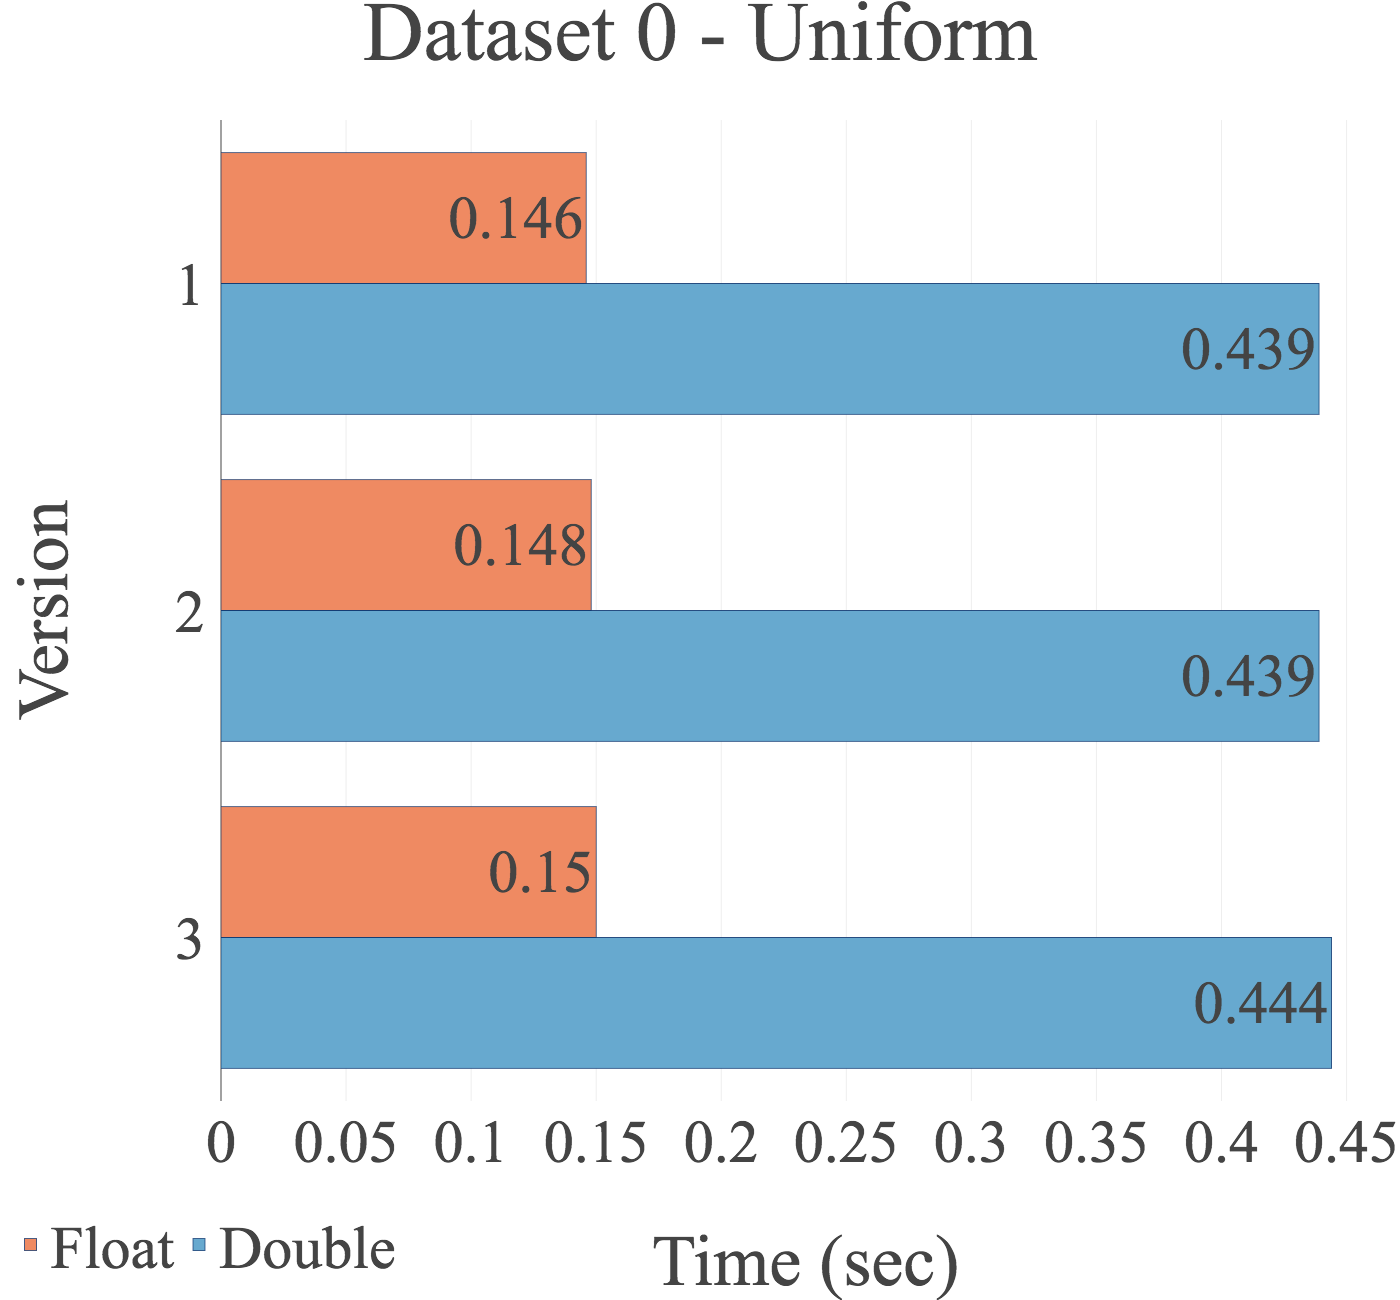
\includegraphics[width=1\textwidth]{img/experiments/multi-versions-0_UNIFORM.png}
\end{subfigure}
\begin{subfigure}{.62\textwidth}
    \centering
    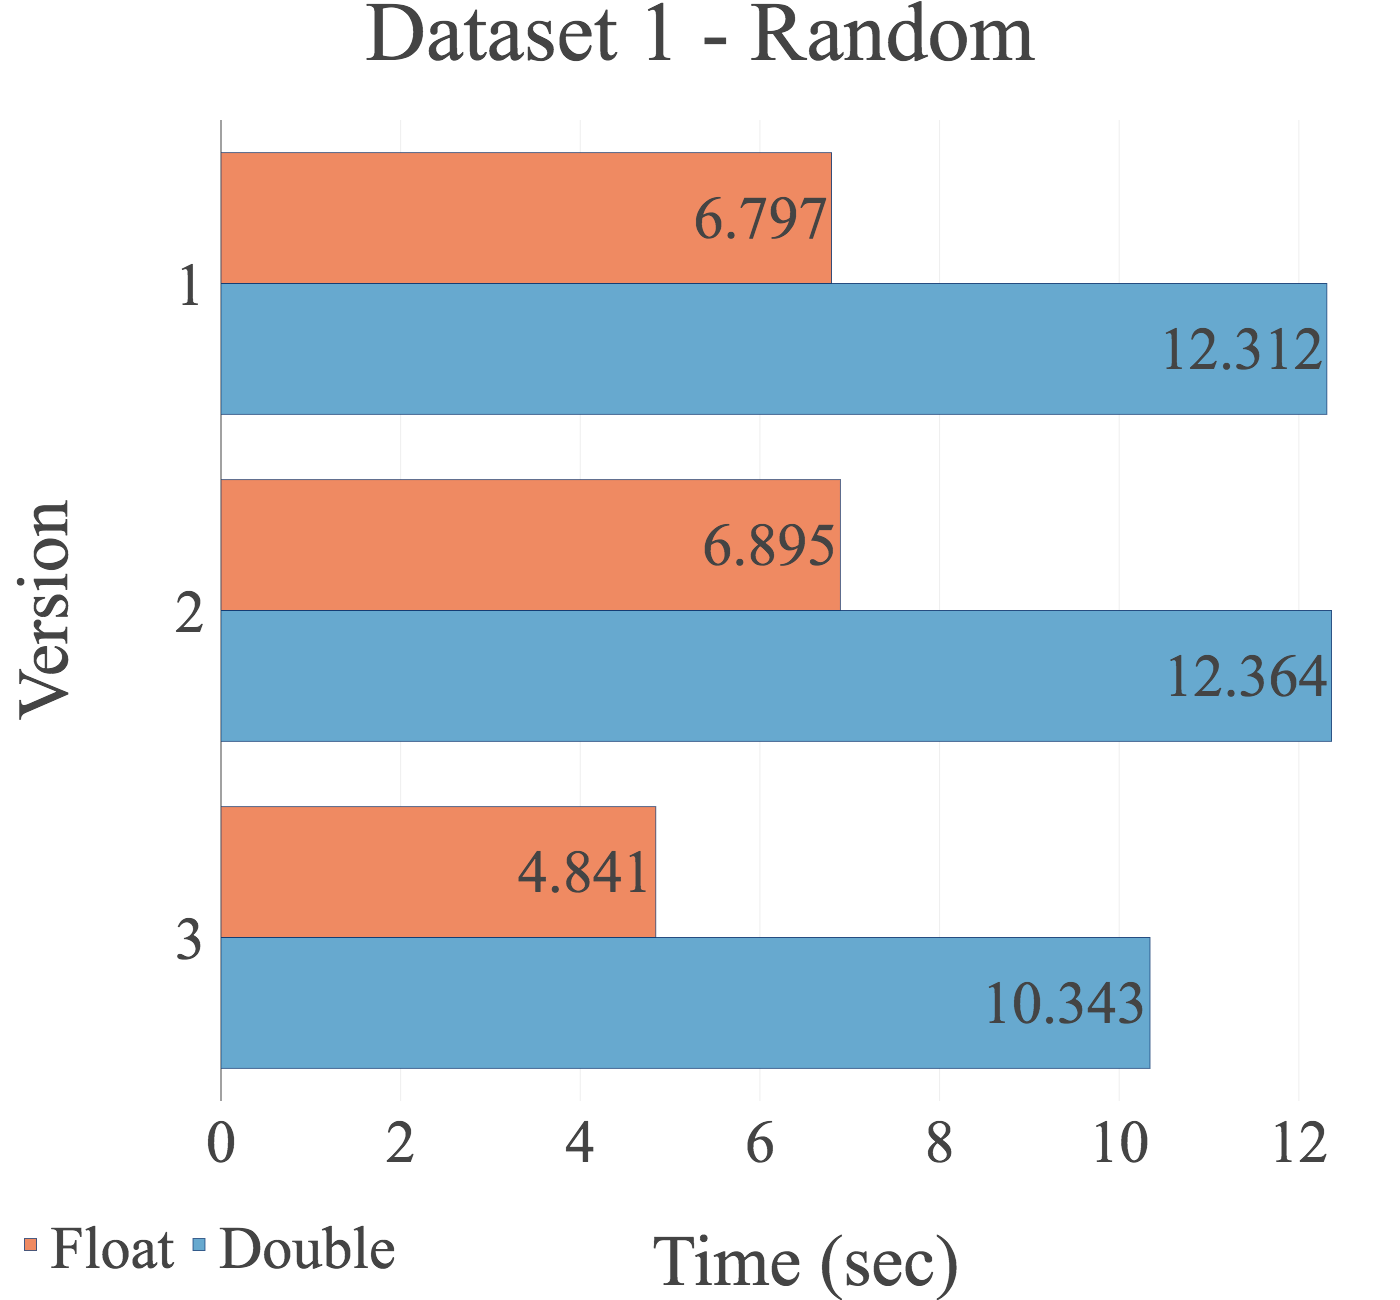
\includegraphics[width=1\textwidth]{img/experiments/multi-versions-1_RAND.png}
\end{subfigure}
\par\bigskip
\par\bigskip
\begin{subfigure}{.62\textwidth}
  \centering
  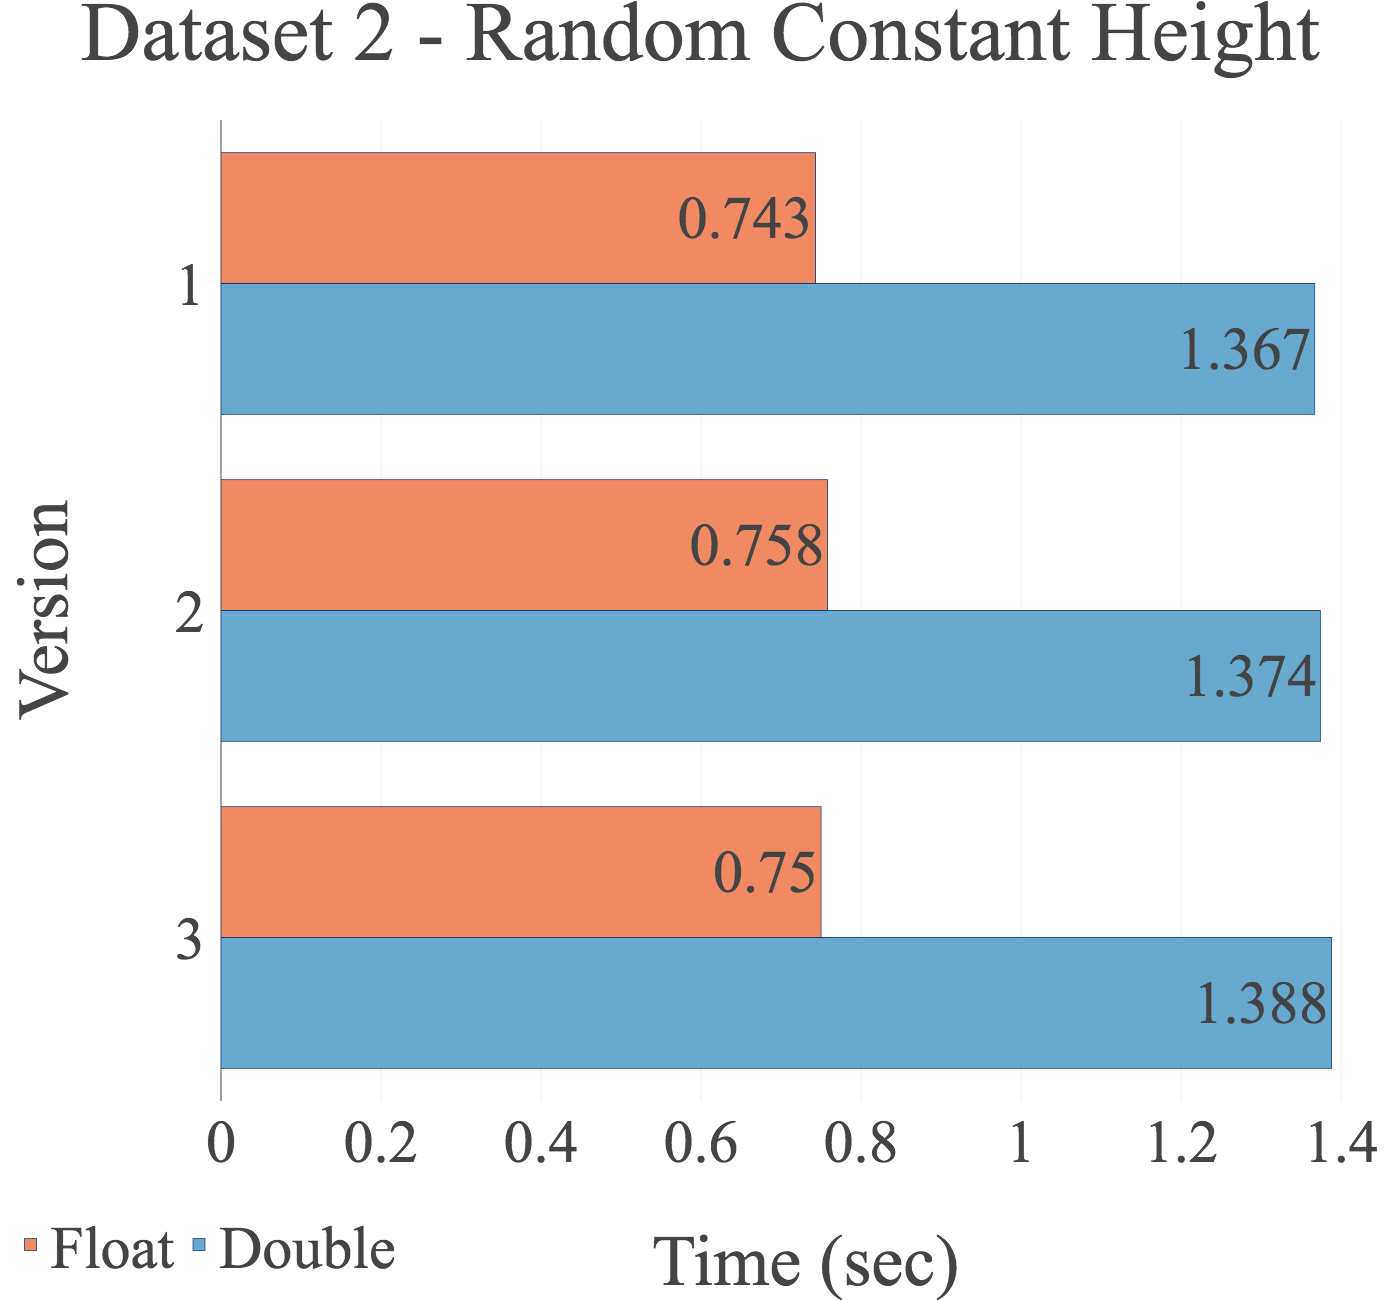
\includegraphics[width=1\textwidth]{img/experiments/multi-versions-2_RANDCONSTHEIGHT.png}
\end{subfigure}
\begin{subfigure}{.62\textwidth}
  \centering
  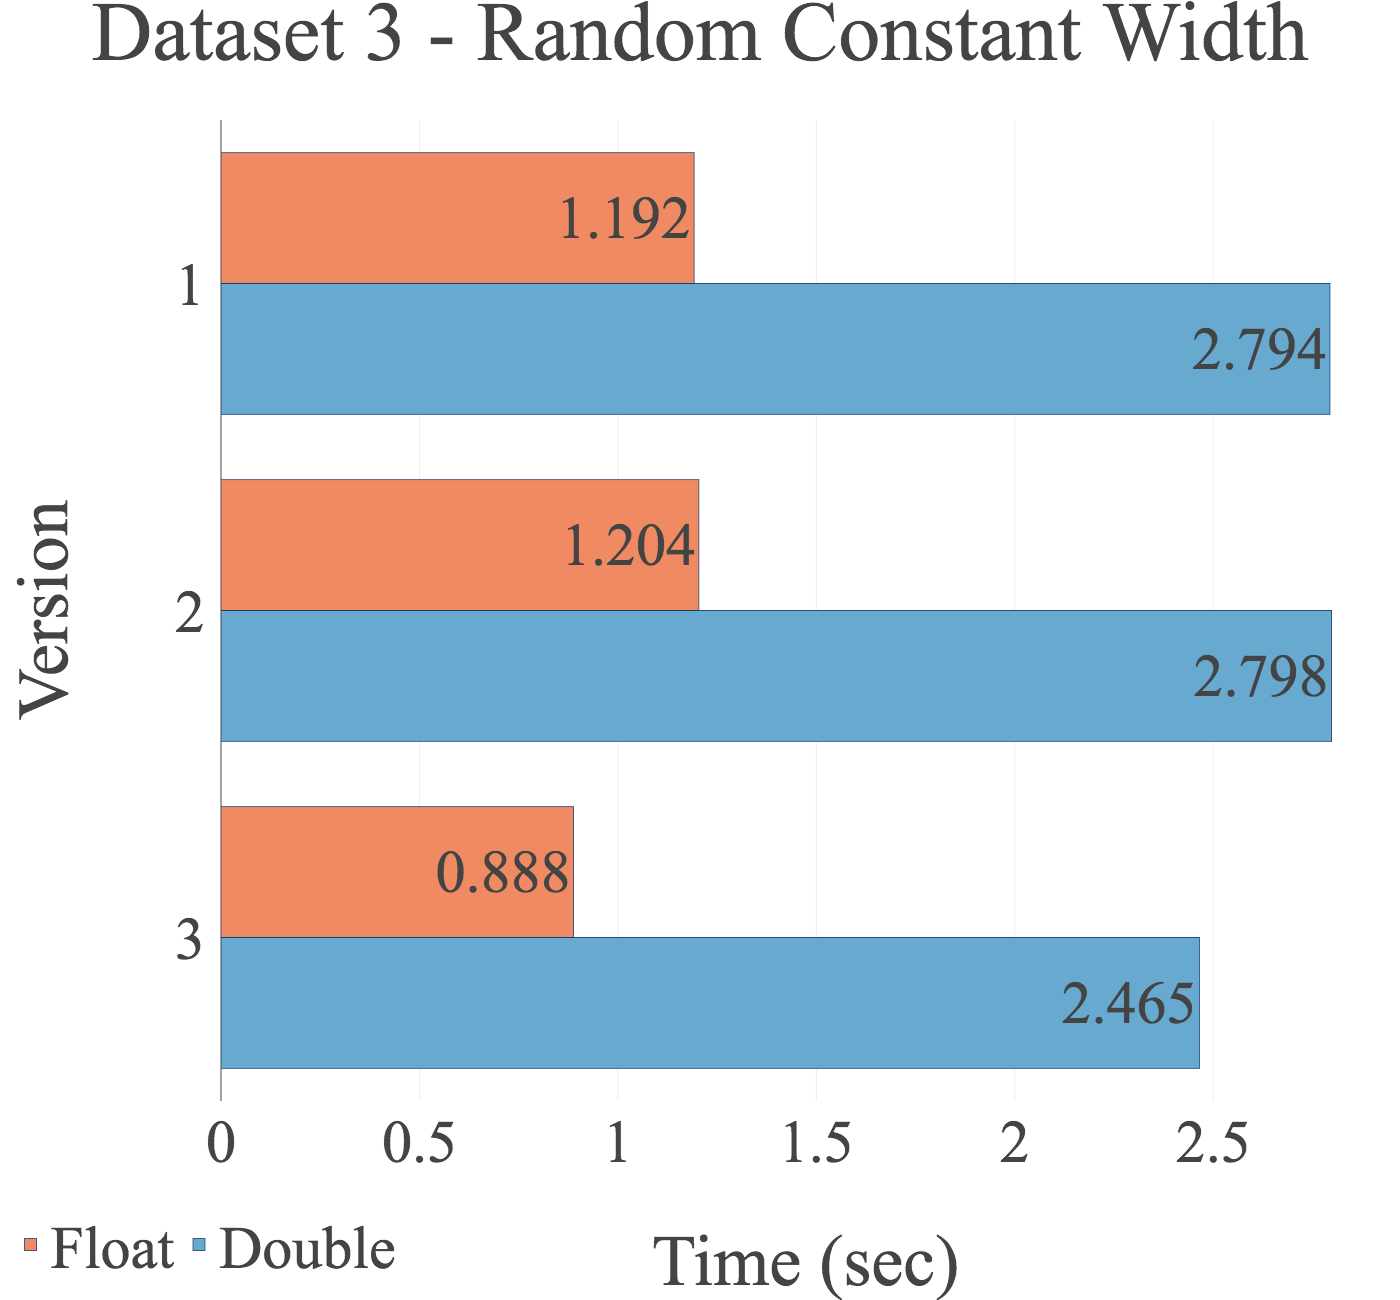
\includegraphics[width=1\textwidth]{img/experiments/multi-versions-3_RANDCONSTWIDTH.png}
\end{subfigure}
\end{adjustwidth}
\end{figure}

\begin{figure}[H]
\begin{adjustwidth}{-2cm}{-2cm}
\begin{subfigure}{.62\textwidth}
  \centering
  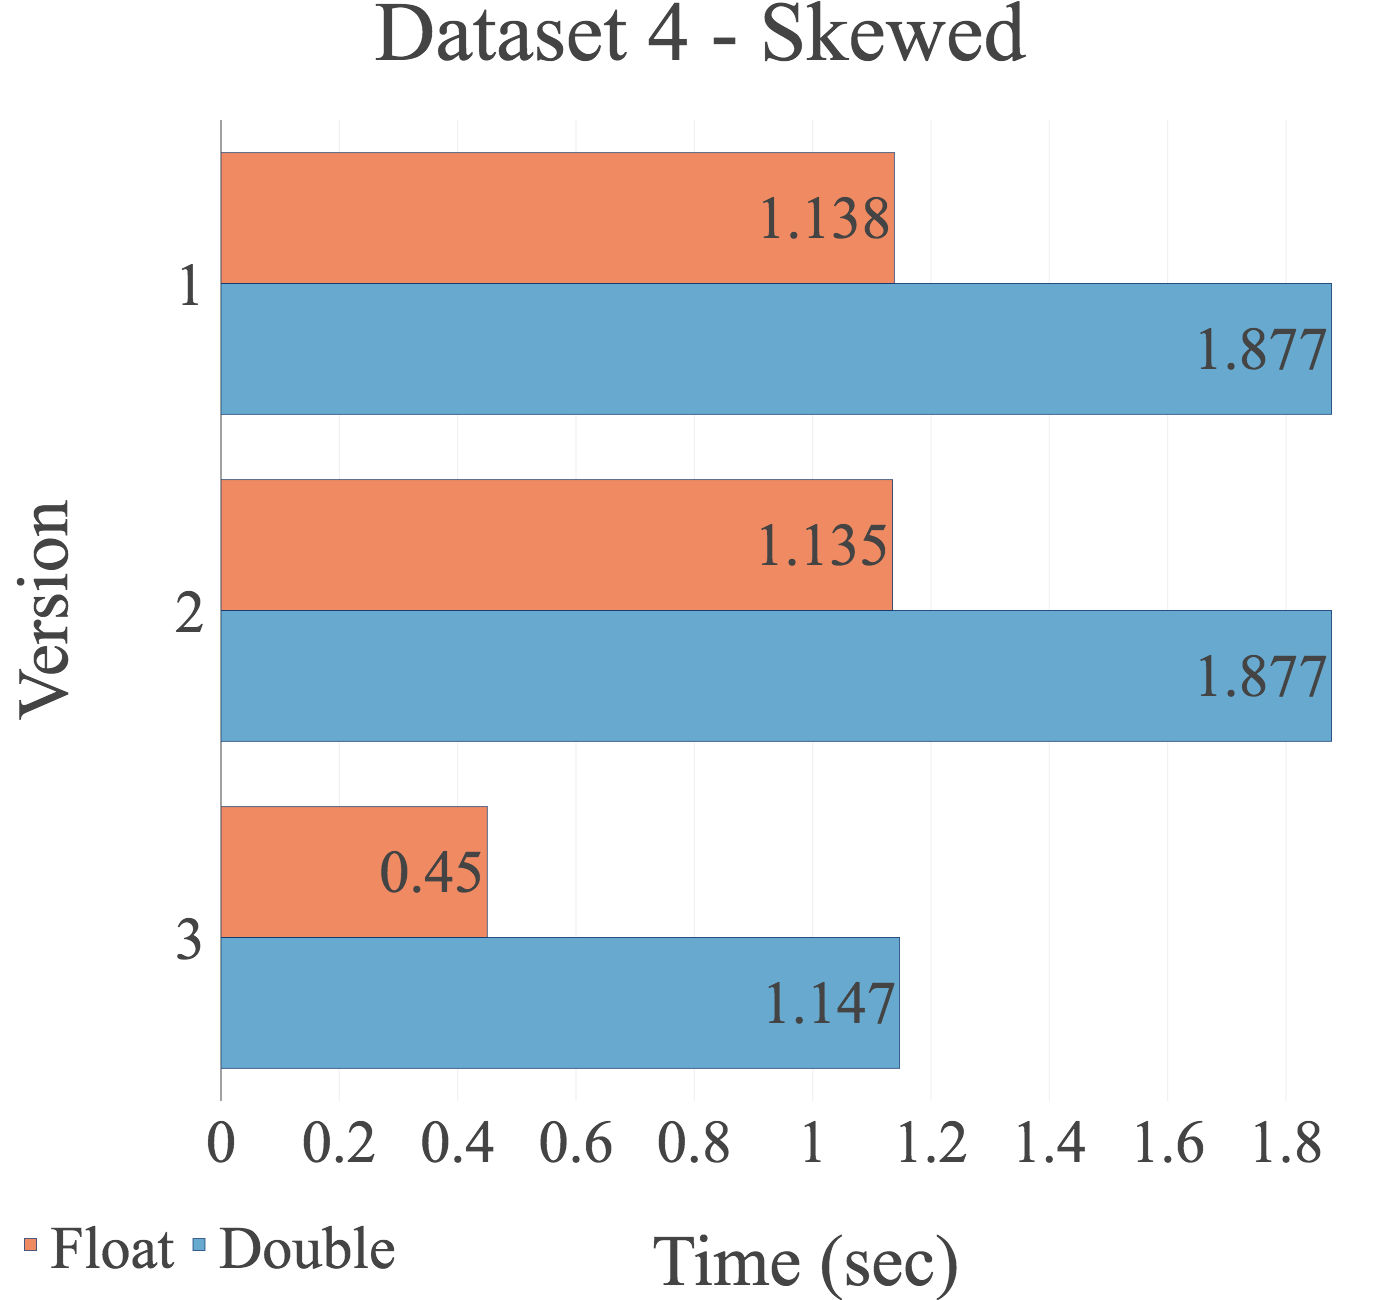
\includegraphics[width=1\textwidth]{img/experiments/multi-versions-4_SKEWED.png}
\end{subfigure}
\begin{subfigure}{.62\textwidth}
  \centering
  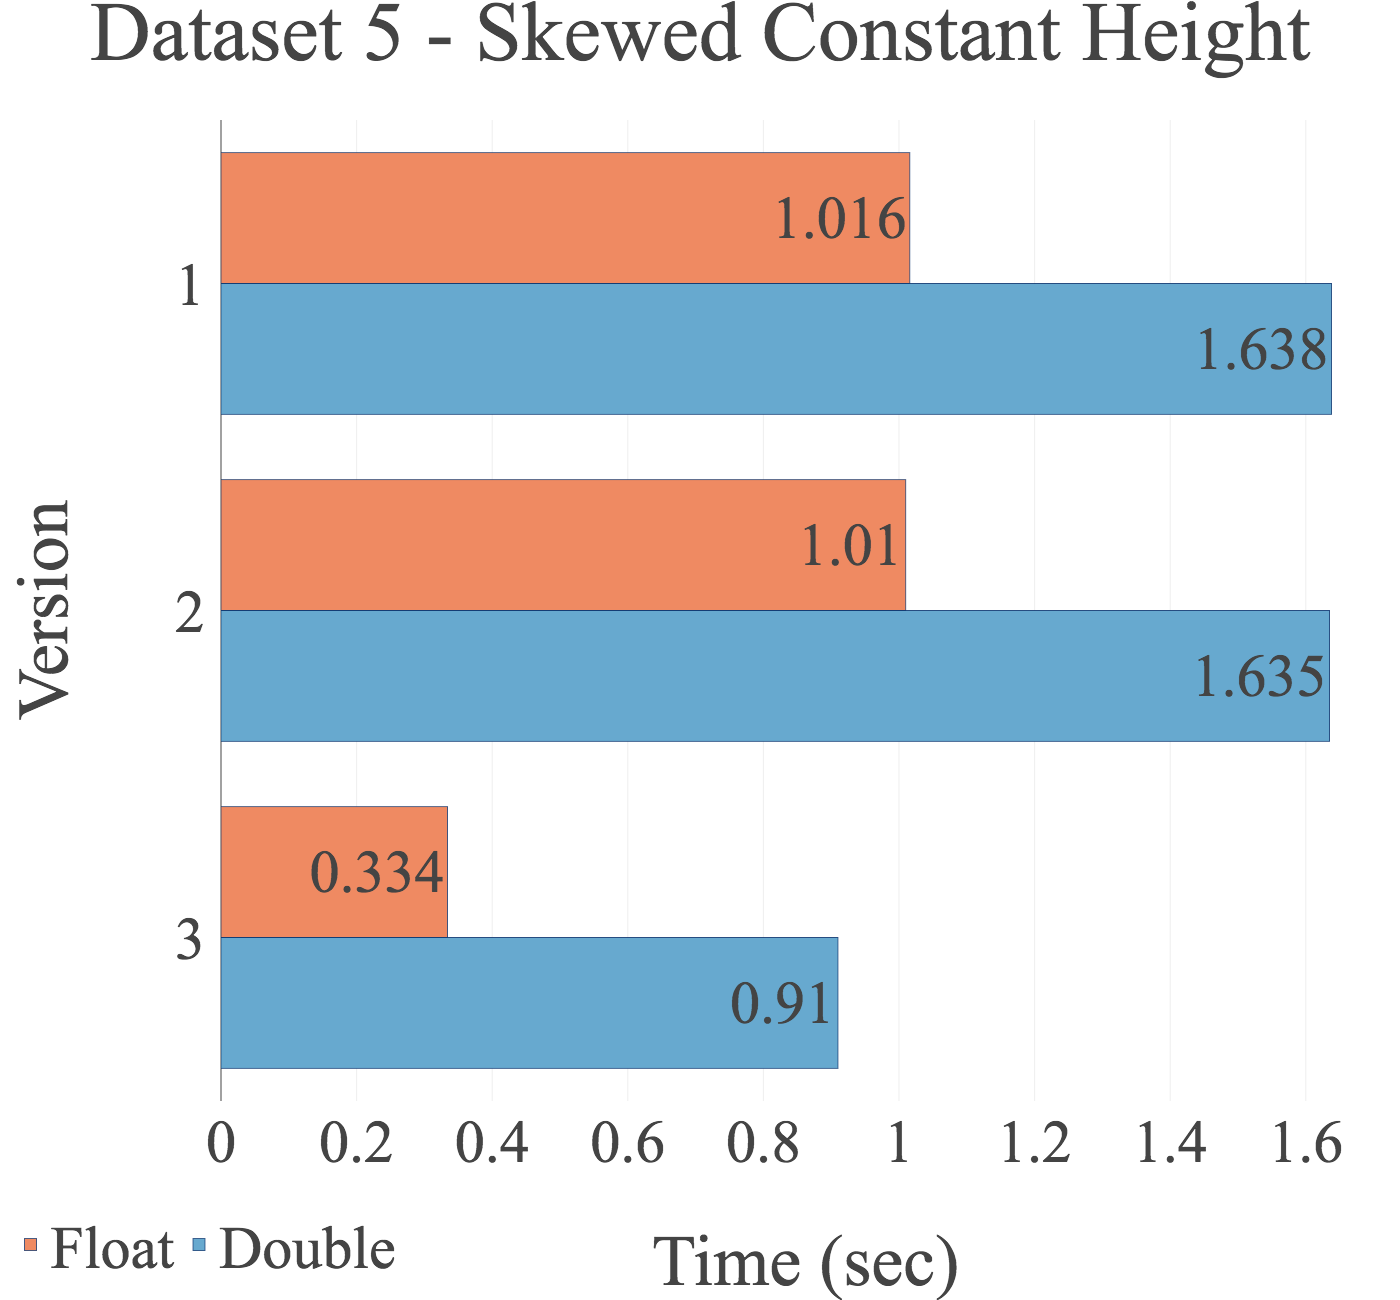
\includegraphics[width=1\textwidth]{img/experiments/multi-versions-5_SKEWEDCONSTHEIGHT.png}
\end{subfigure}
\par\bigskip
\par\bigskip
\centering
\begin{subfigure}{.62\textwidth}
  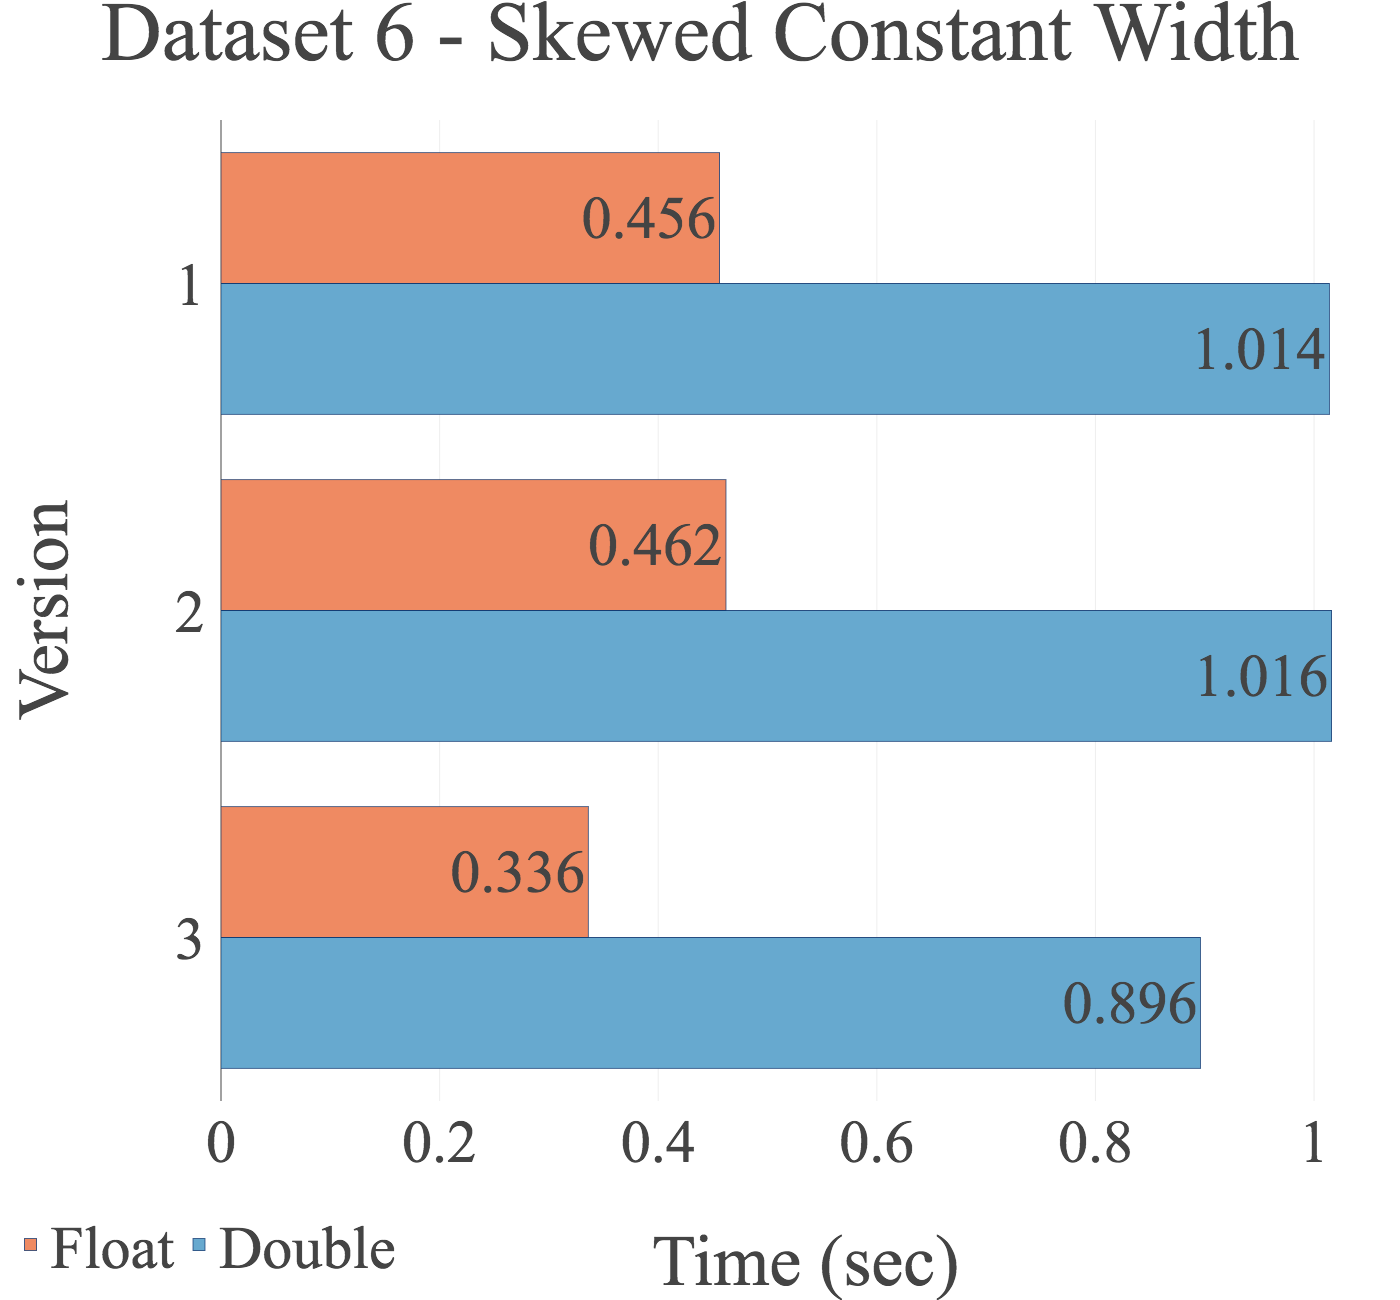
\includegraphics[width=1\textwidth]{img/experiments/multi-versions-6_SKEWEDCONSTWIDTH.png}
\end{subfigure}
\end{adjustwidth}
\end{figure}

% SECTION END %


% SECTION START %
\section{Block Size Experiments (Best Runtimes)}
\label{appendix:option:block}
\begin{figure}[H]
\begin{adjustwidth}{-2cm}{-2cm}
\centering
\begin{subfigure}{.62\textwidth}
    \centering
    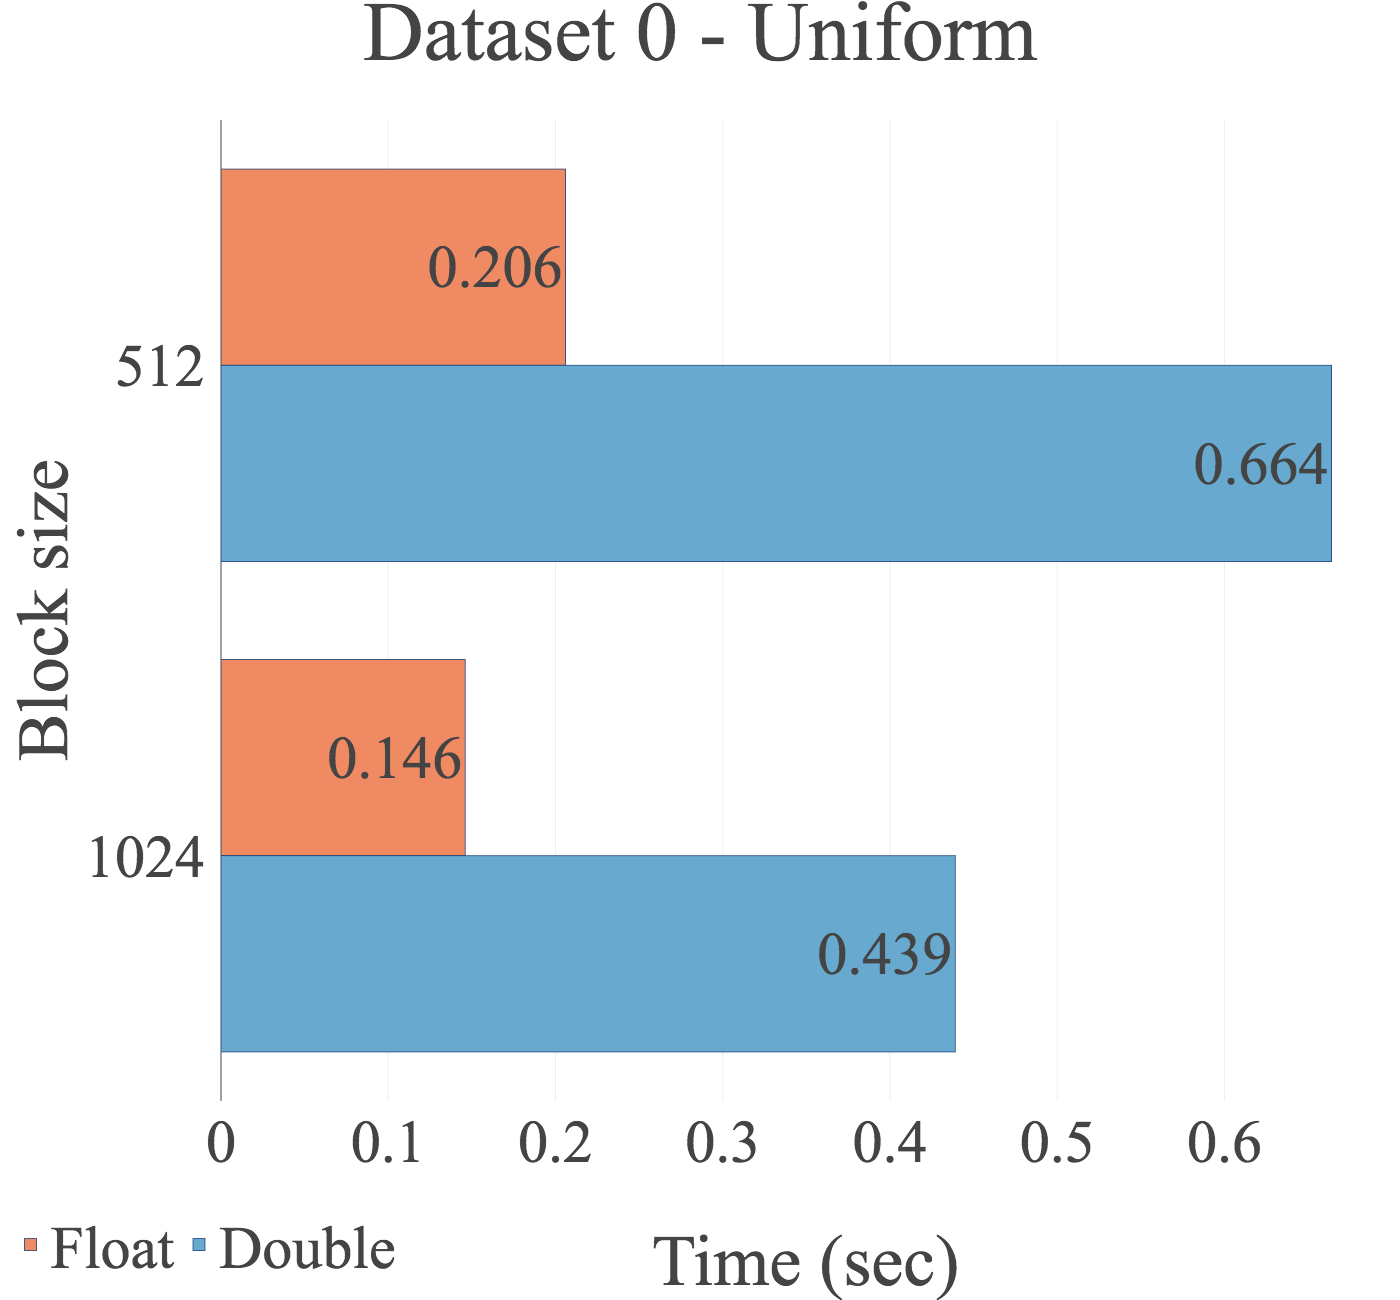
\includegraphics[width=1\textwidth]{img/experiments/multi-blocks-0_UNIFORM.png}
\end{subfigure}
\begin{subfigure}{.62\textwidth}
    \centering
    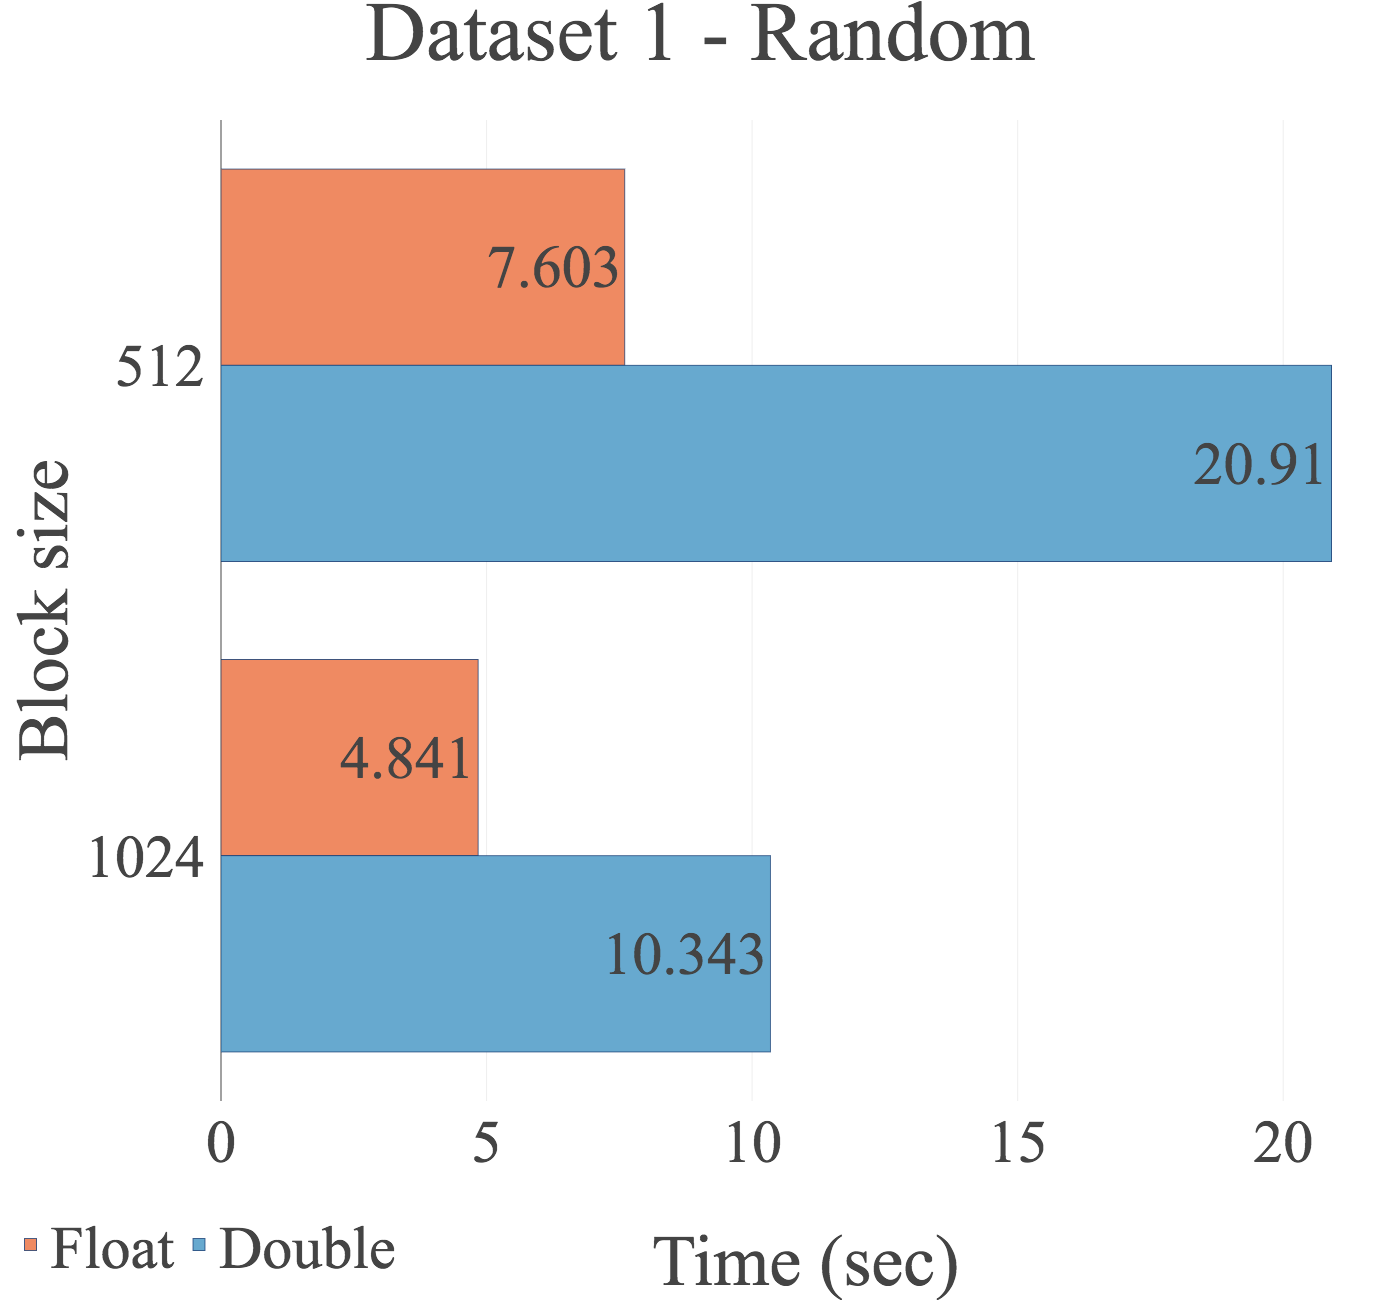
\includegraphics[width=1\textwidth]{img/experiments/multi-blocks-1_RAND.png}
\end{subfigure}
\par\bigskip
\par\bigskip
\begin{subfigure}{.62\textwidth}
  \centering
  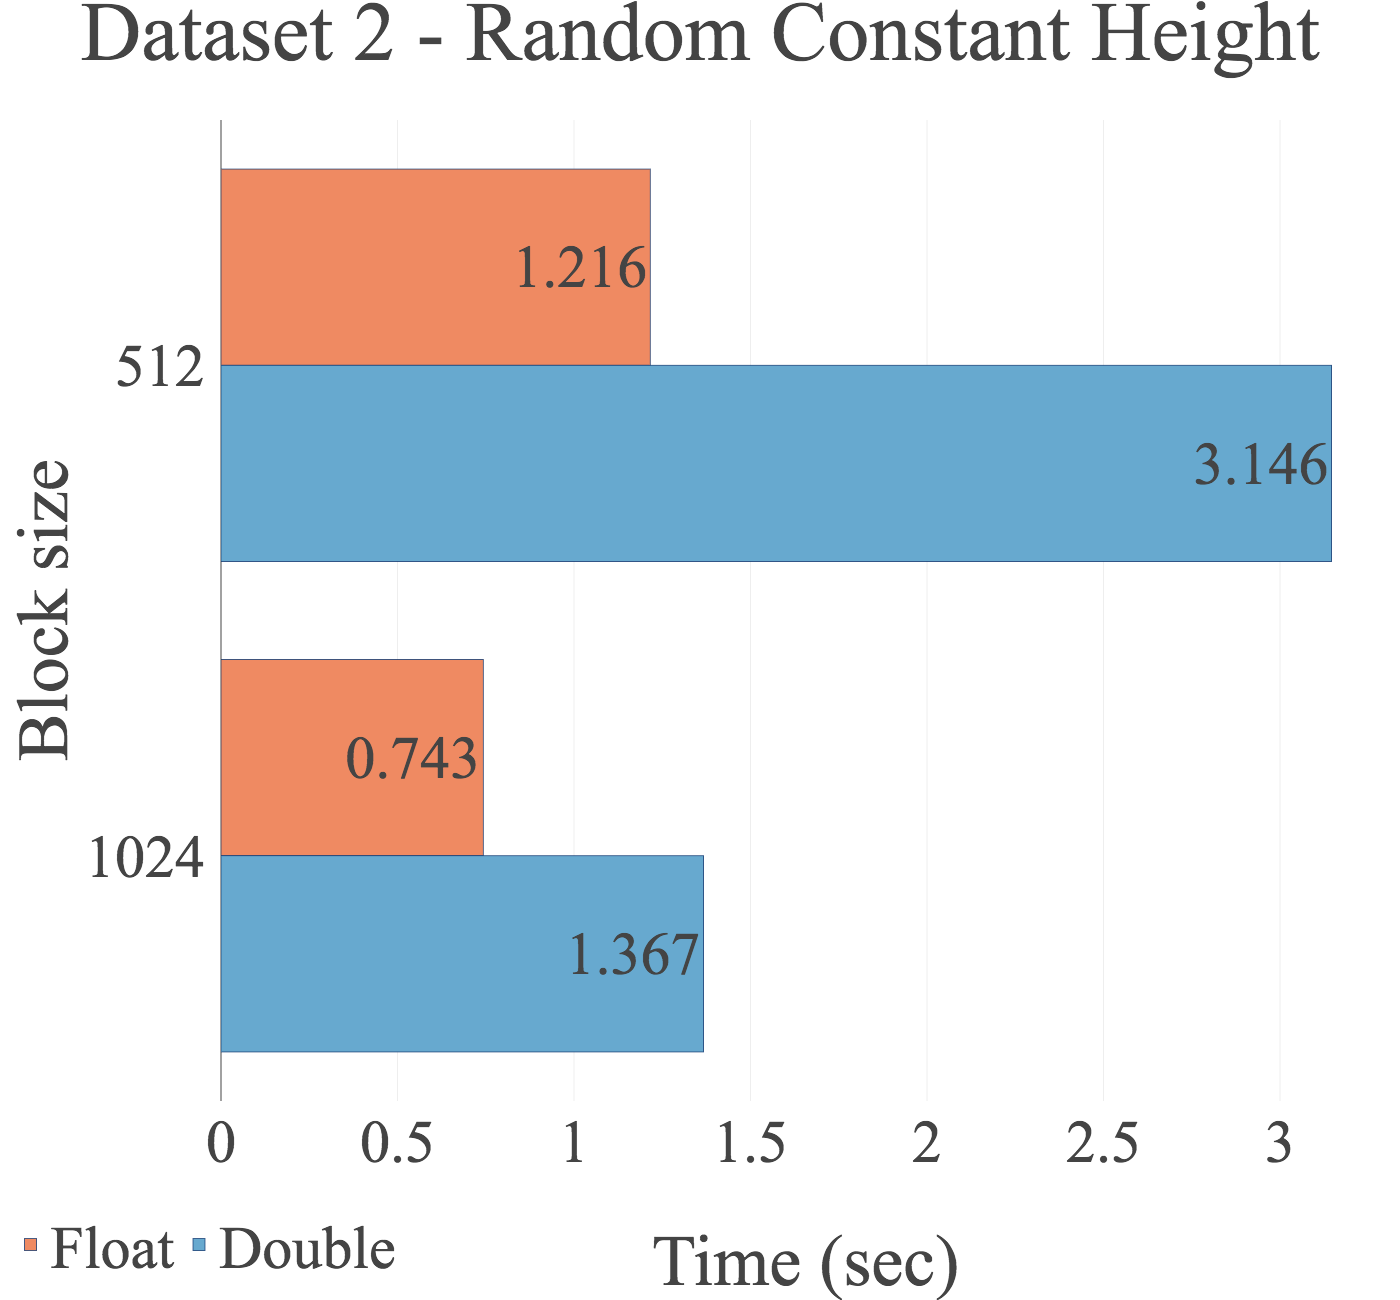
\includegraphics[width=1\textwidth]{img/experiments/multi-blocks-2_RANDCONSTHEIGHT.png}
\end{subfigure}
\begin{subfigure}{.62\textwidth}
  \centering
  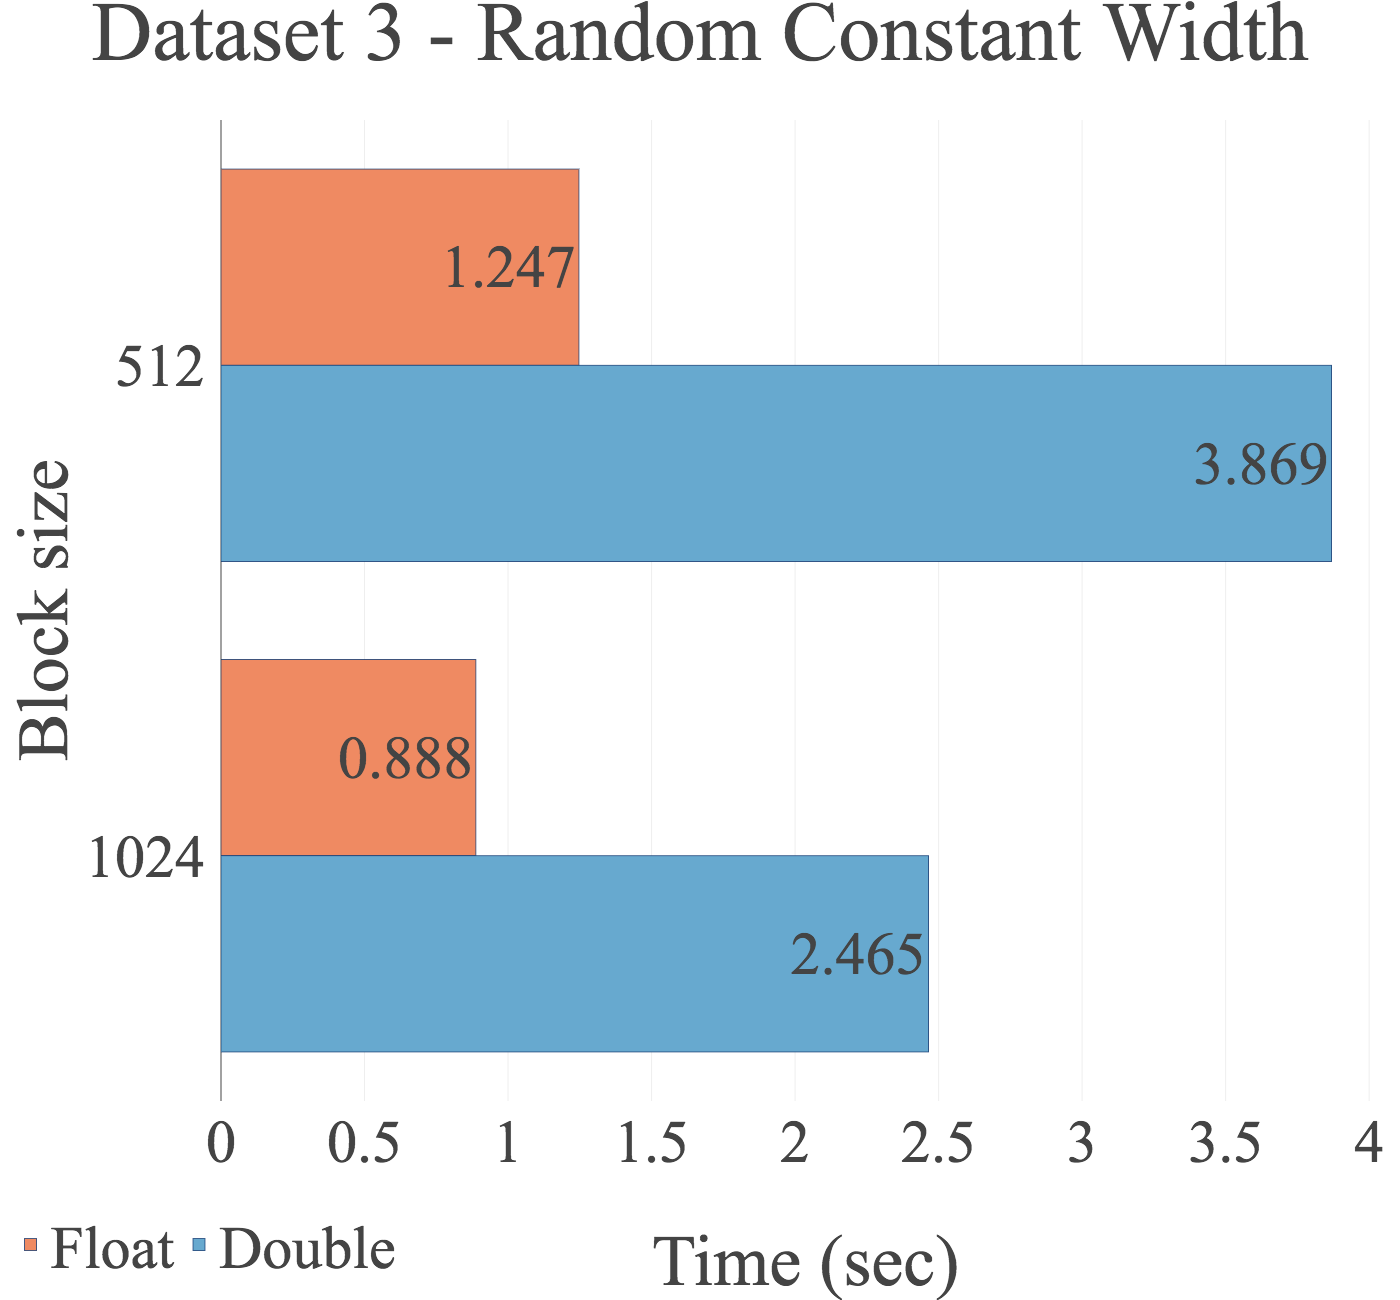
\includegraphics[width=1\textwidth]{img/experiments/multi-blocks-3_RANDCONSTWIDTH.png}
\end{subfigure}
\end{adjustwidth}
\end{figure}

\begin{figure}[H]
\begin{adjustwidth}{-2cm}{-2cm}
\begin{subfigure}{.62\textwidth}
  \centering
  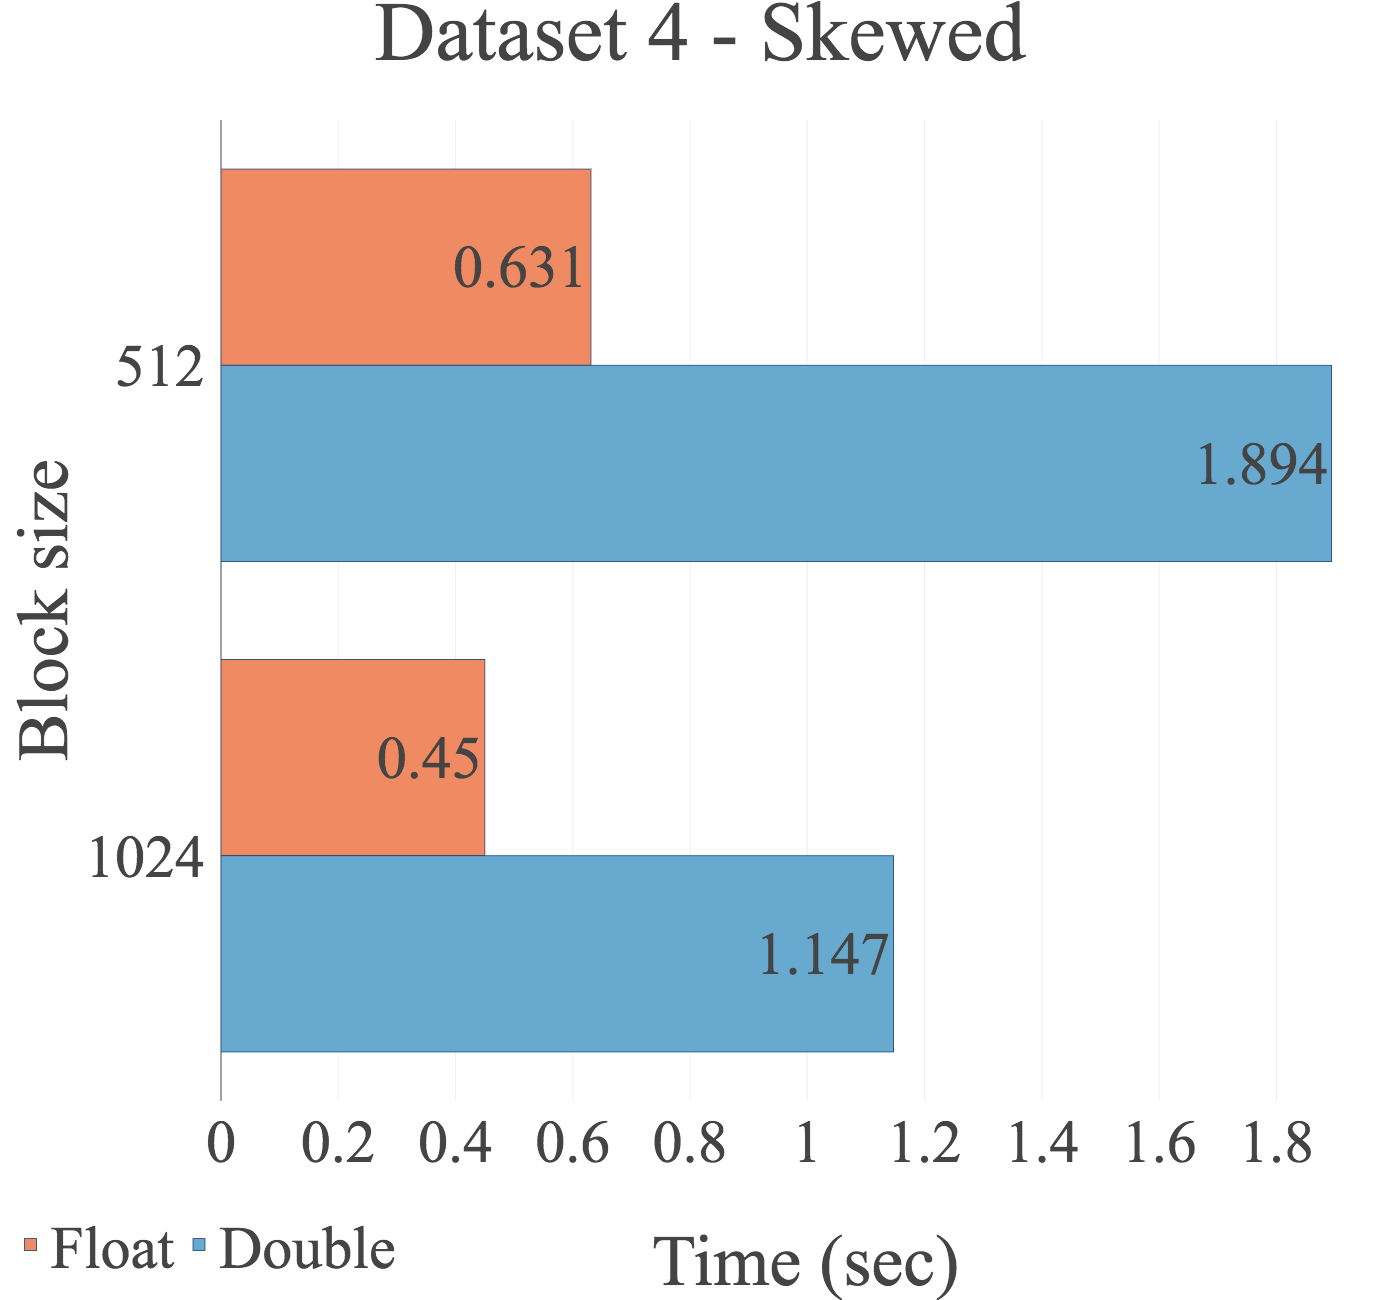
\includegraphics[width=1\textwidth]{img/experiments/multi-blocks-4_SKEWED.png}
\end{subfigure}
\begin{subfigure}{.62\textwidth}
  \centering
  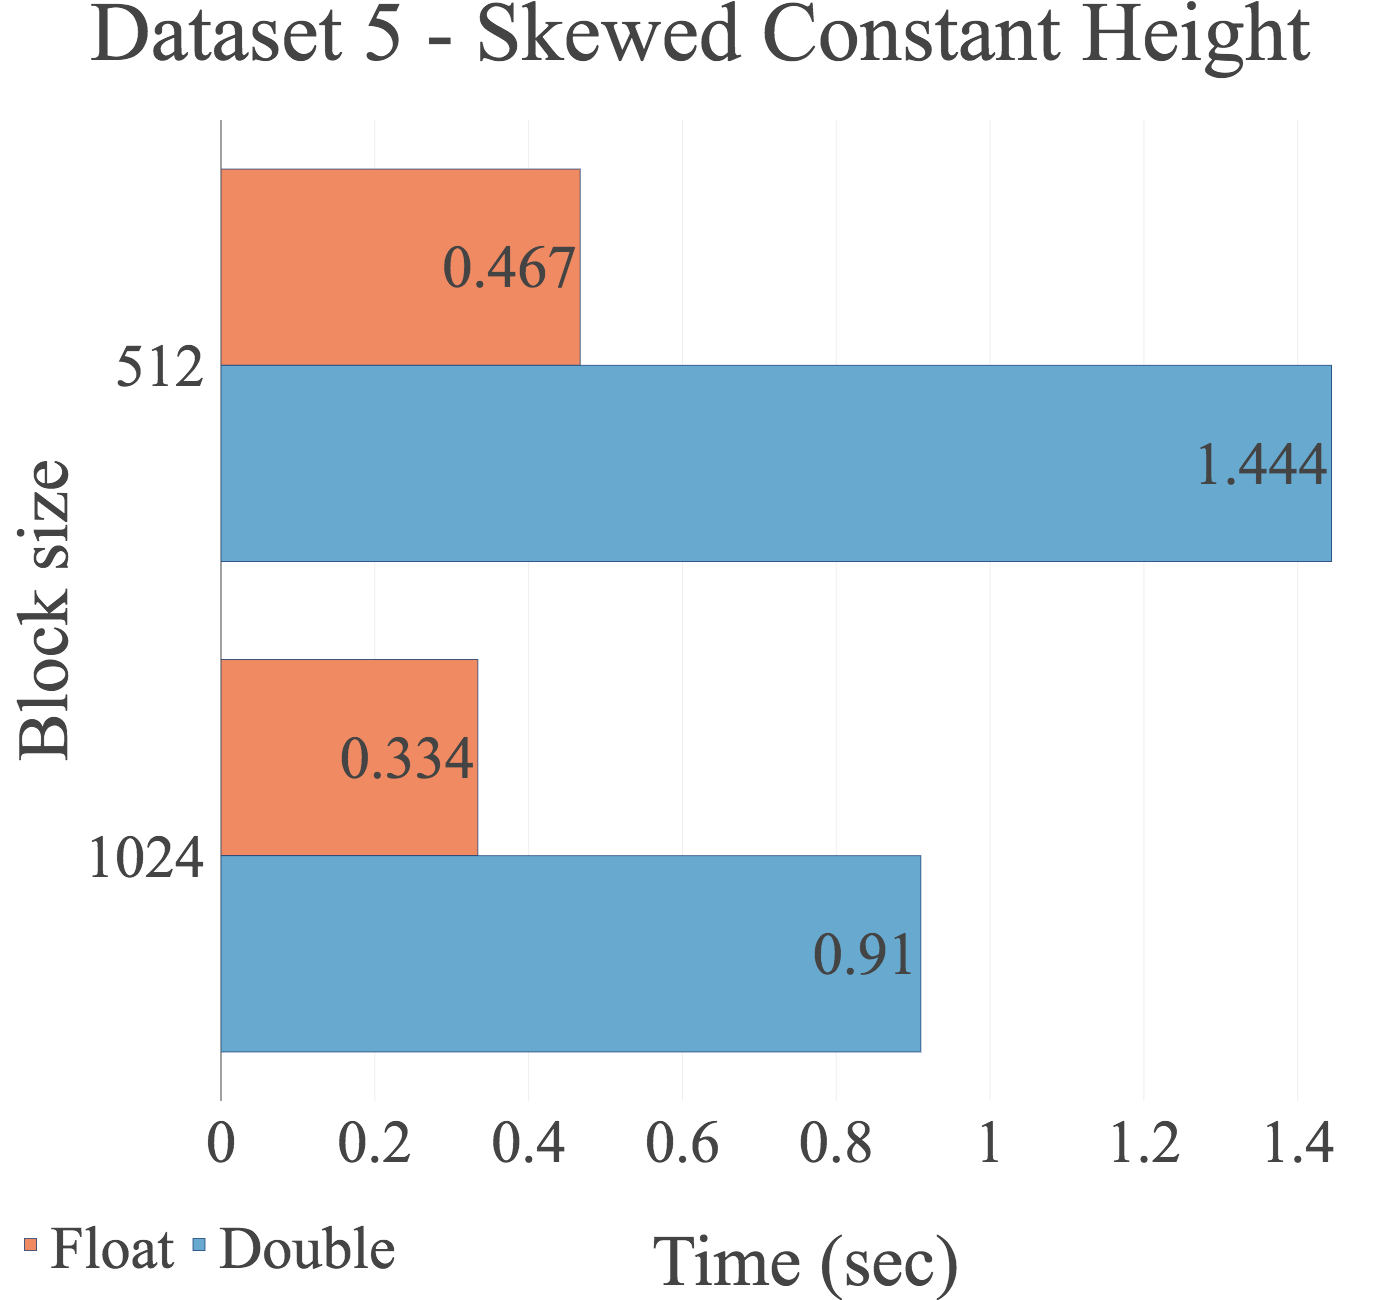
\includegraphics[width=1\textwidth]{img/experiments/multi-blocks-5_SKEWEDCONSTHEIGHT.png}
\end{subfigure}
\par\bigskip
\par\bigskip
\centering
\begin{subfigure}{.62\textwidth}
  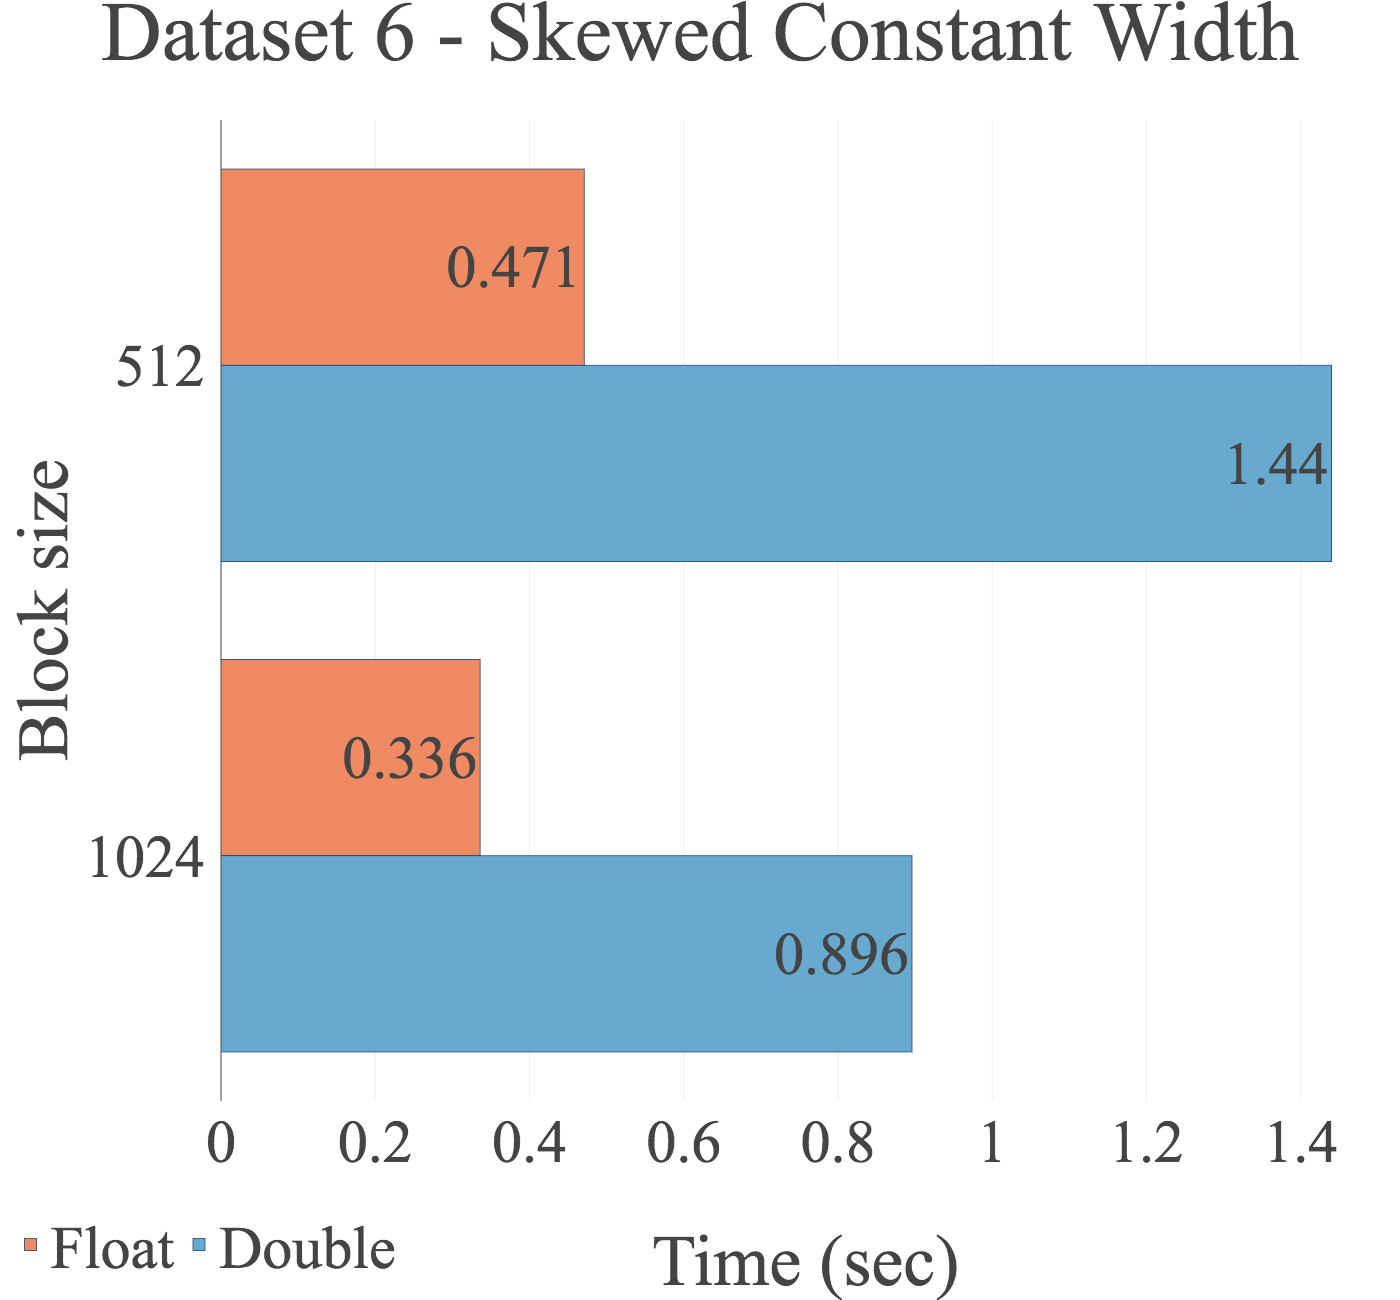
\includegraphics[width=1\textwidth]{img/experiments/multi-blocks-6_SKEWEDCONSTWIDTH.png}
\end{subfigure}
\end{adjustwidth}
\end{figure}

% SECTION END %

% SECTION START %
\section{Sorting Experiments (Best Runtimes)}
\label{appendix:experiments:cudamulti:sorting}
\begin{figure}[H]
\begin{adjustwidth}{-2cm}{-2cm}
\centering
\begin{subfigure}{.62\textwidth}
    \centering
    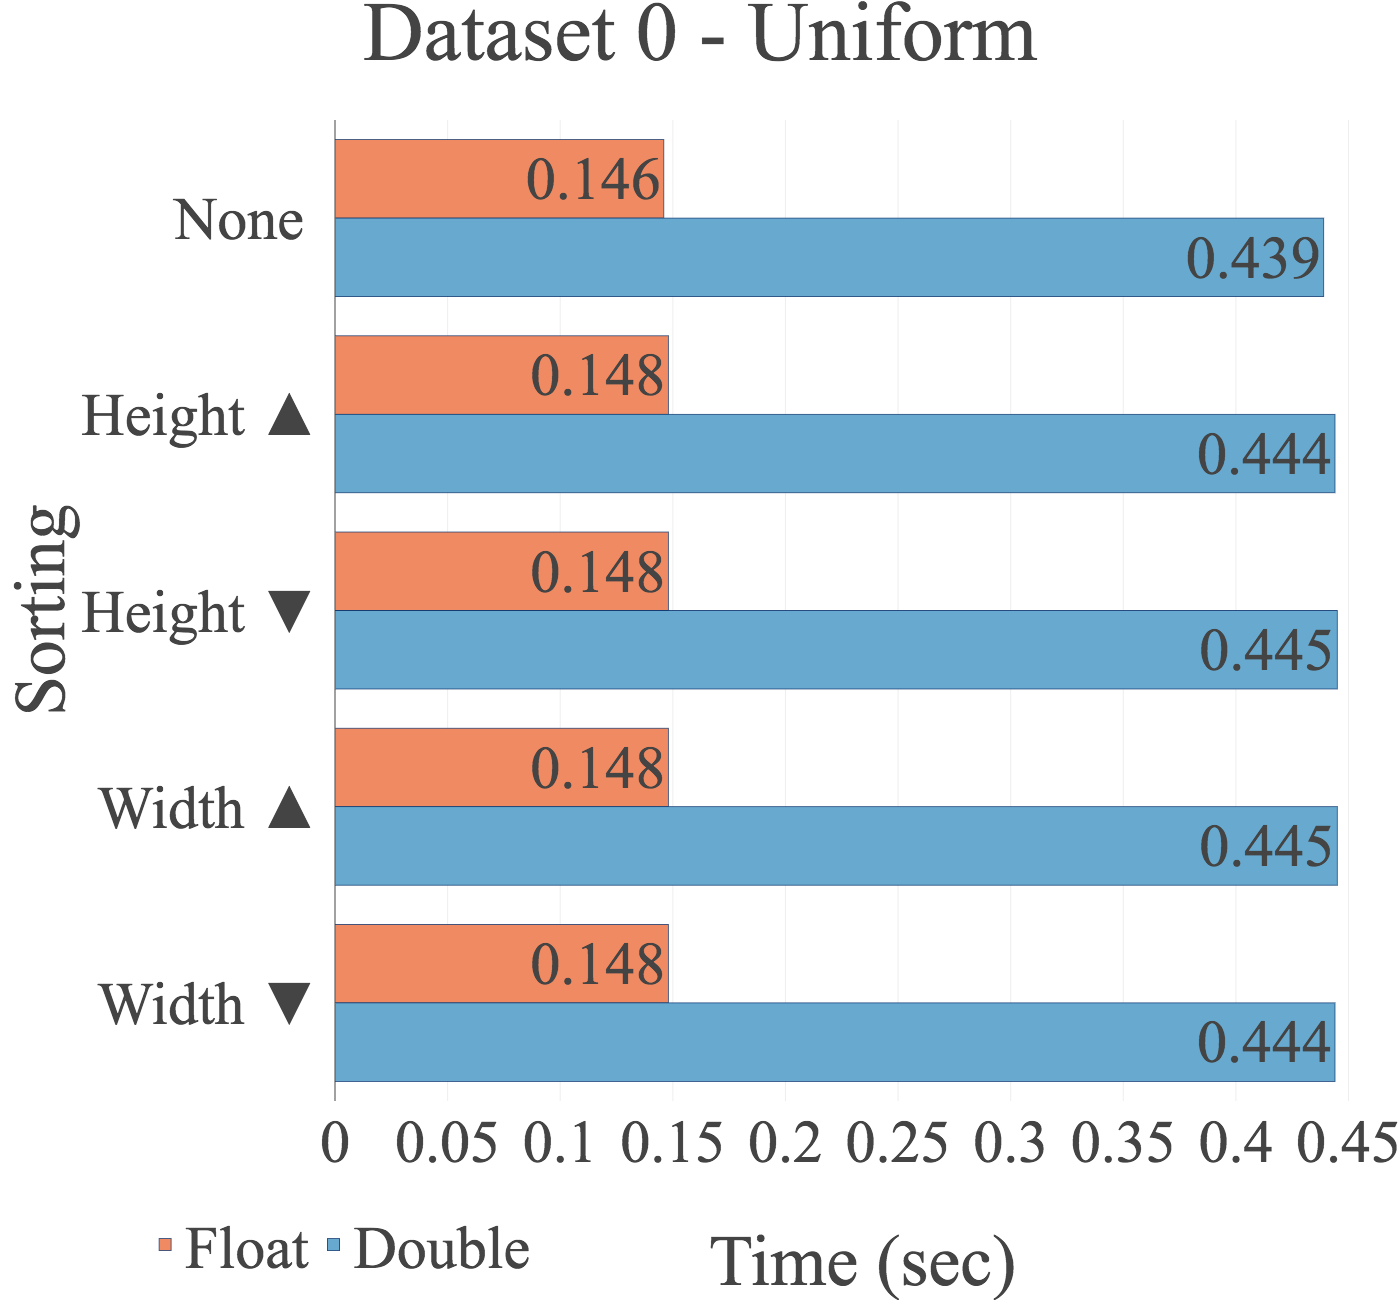
\includegraphics[width=1\textwidth]{img/experiments/multi-sorts-0_UNIFORM.png}
\end{subfigure}
\begin{subfigure}{.62\textwidth}
    \centering
    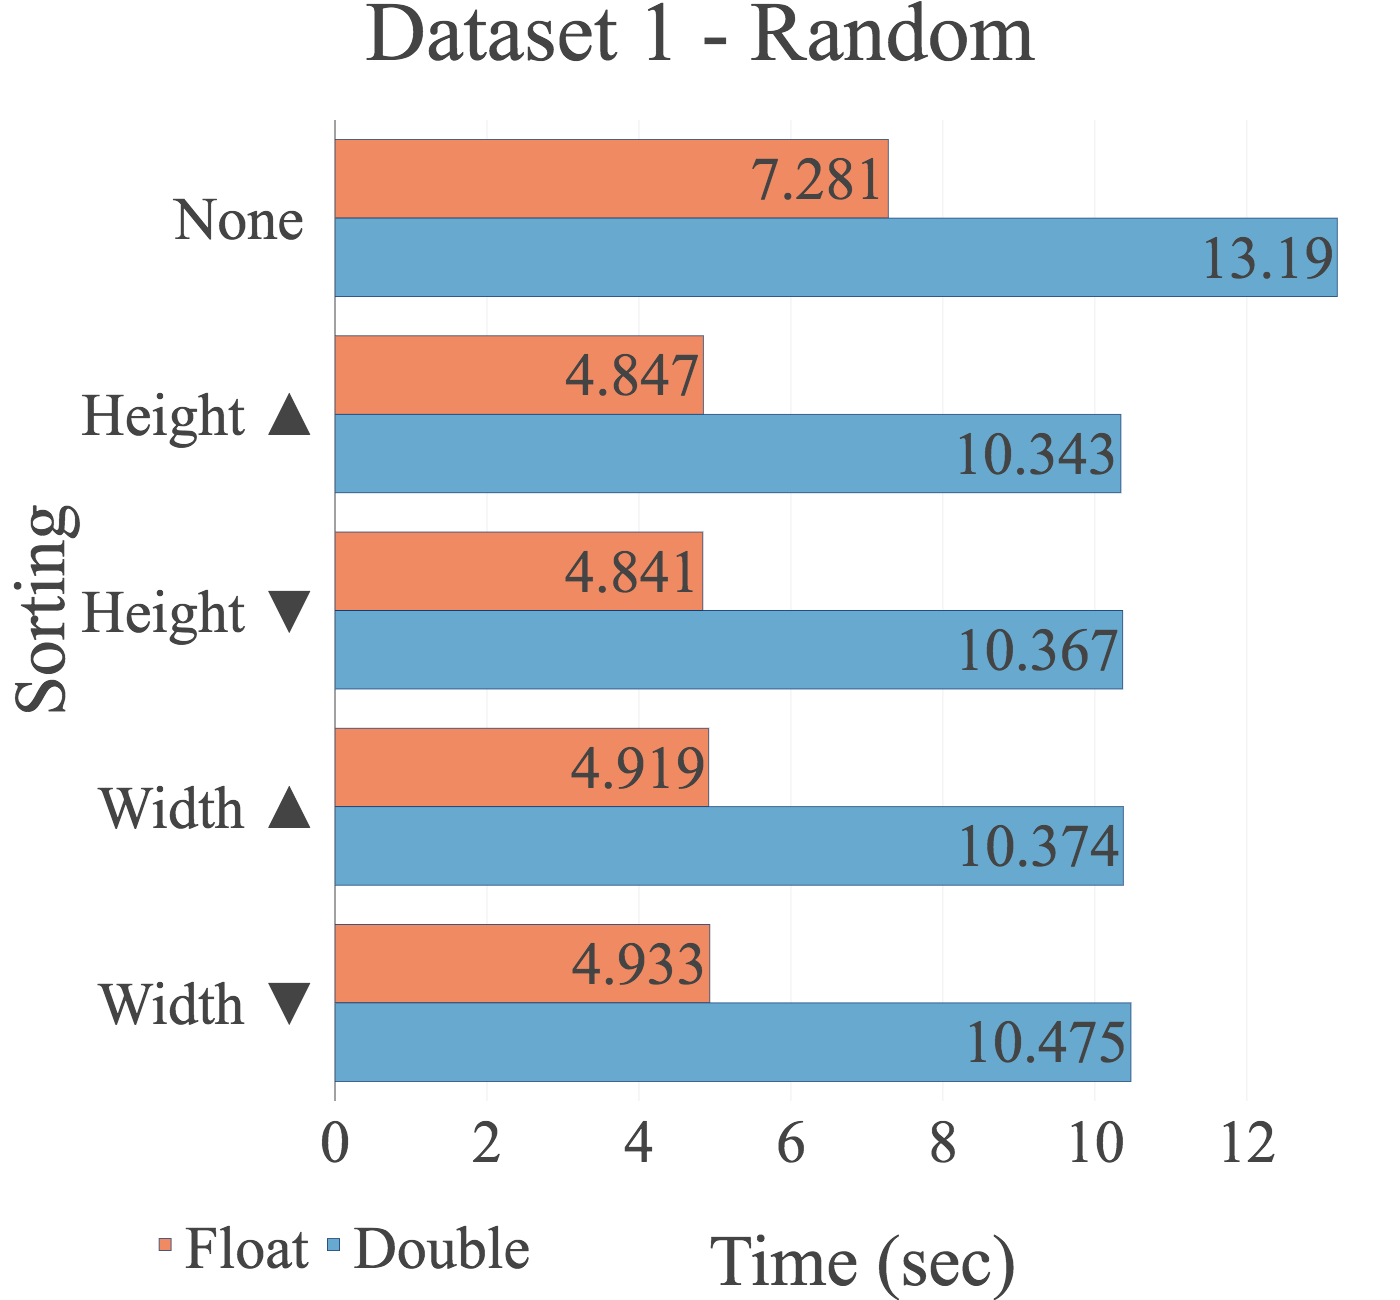
\includegraphics[width=1\textwidth]{img/experiments/multi-sorts-1_RAND.png}
\end{subfigure}
\par\bigskip
\par\bigskip
\begin{subfigure}{.62\textwidth}
  \centering
  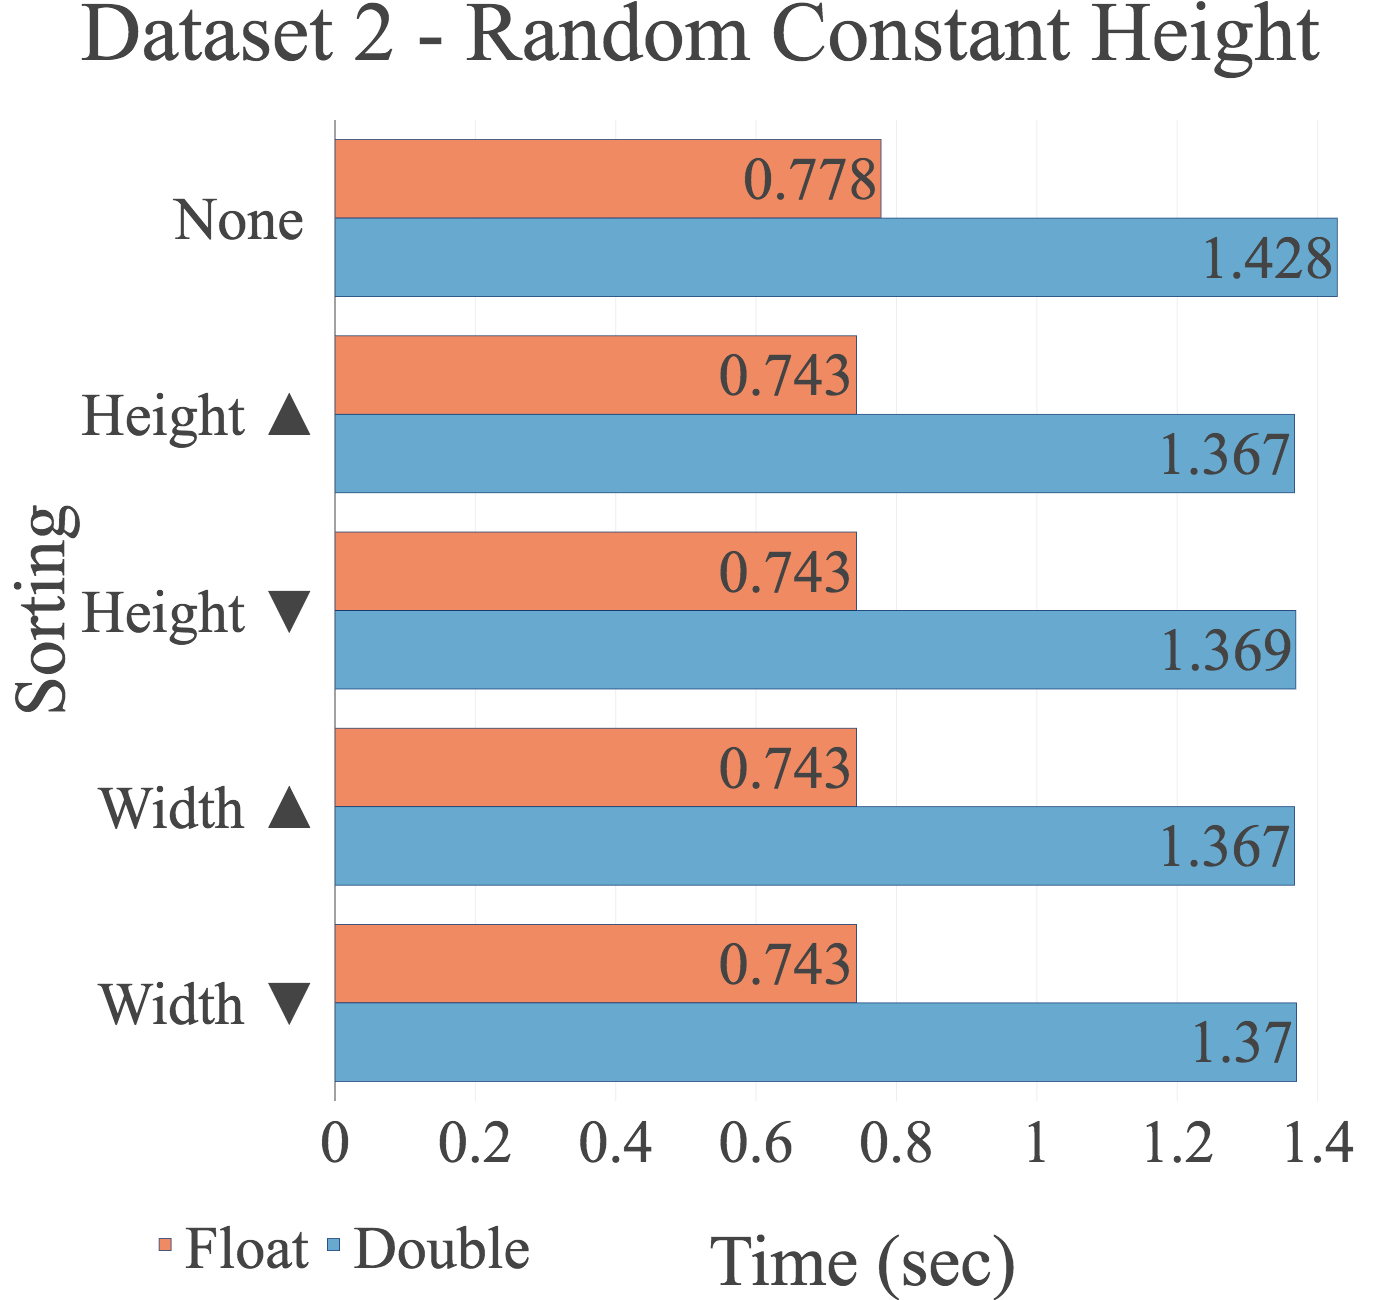
\includegraphics[width=1\textwidth]{img/experiments/multi-sorts-2_RANDCONSTHEIGHT.png}
\end{subfigure}
\begin{subfigure}{.62\textwidth}
  \centering
  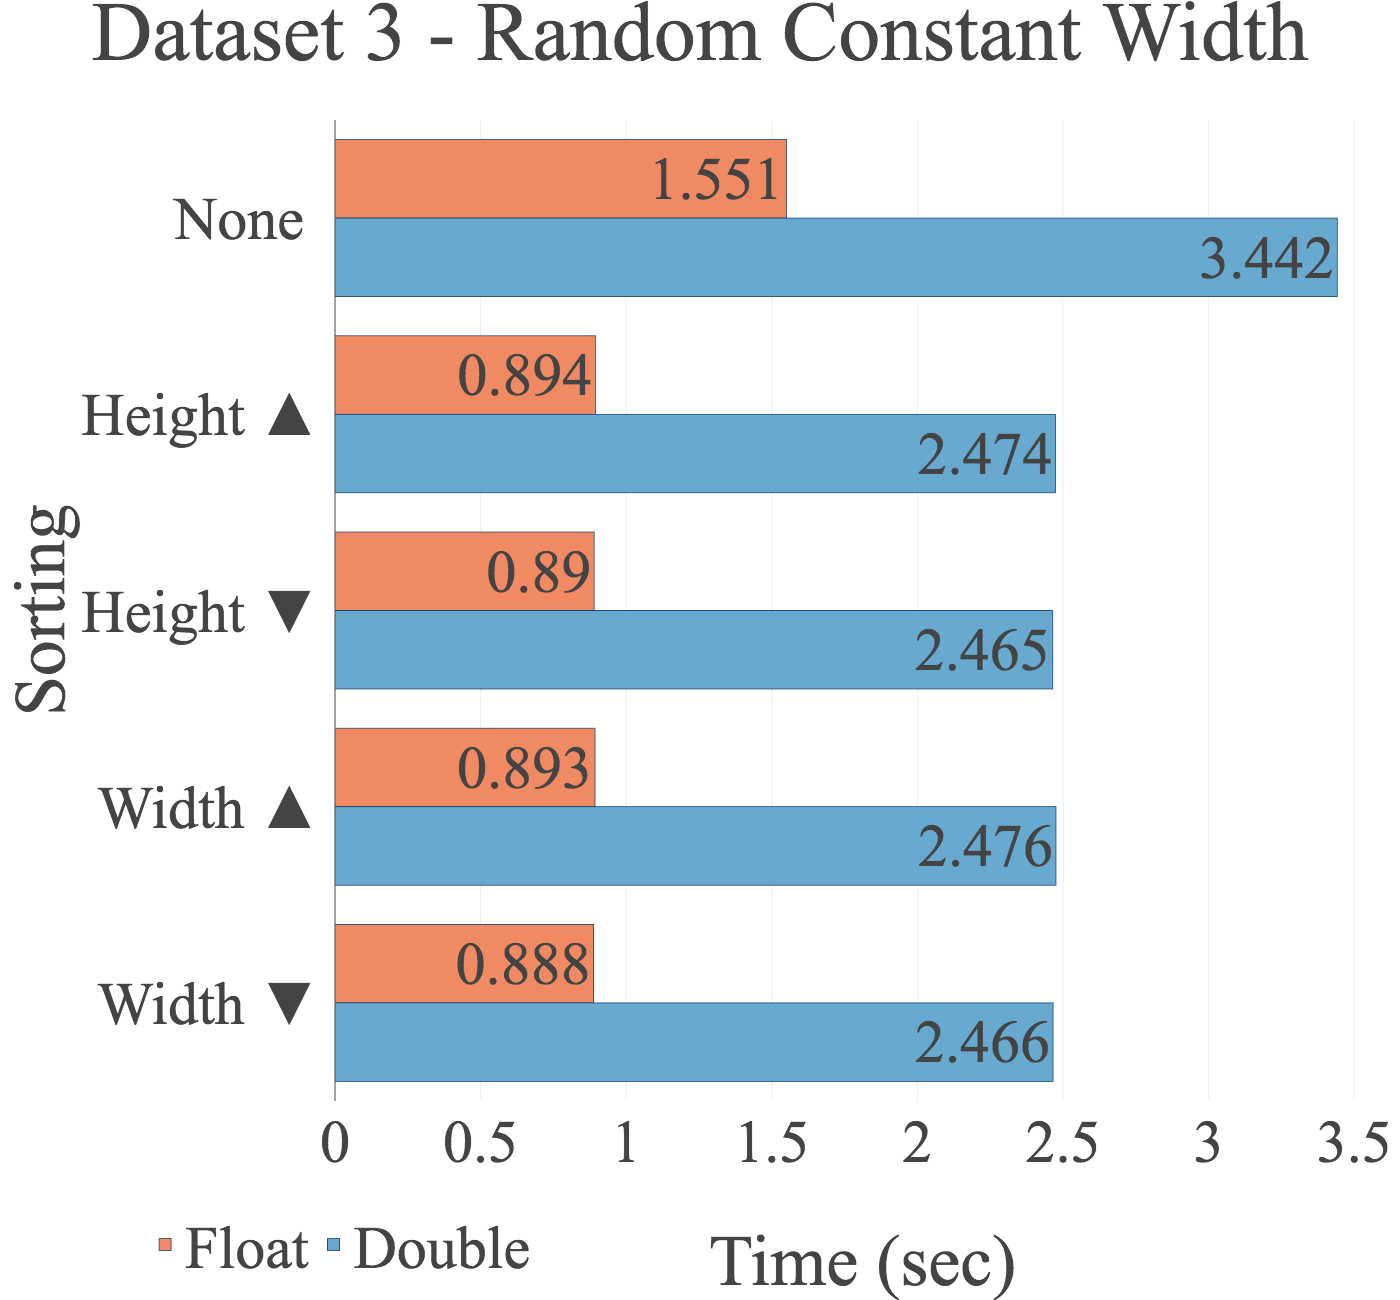
\includegraphics[width=1\textwidth]{img/experiments/multi-sorts-3_RANDCONSTWIDTH.png}
\end{subfigure}
\end{adjustwidth}
\end{figure}

\begin{figure}[H]
\begin{adjustwidth}{-2cm}{-2cm}
\begin{subfigure}{.62\textwidth}
  \centering
  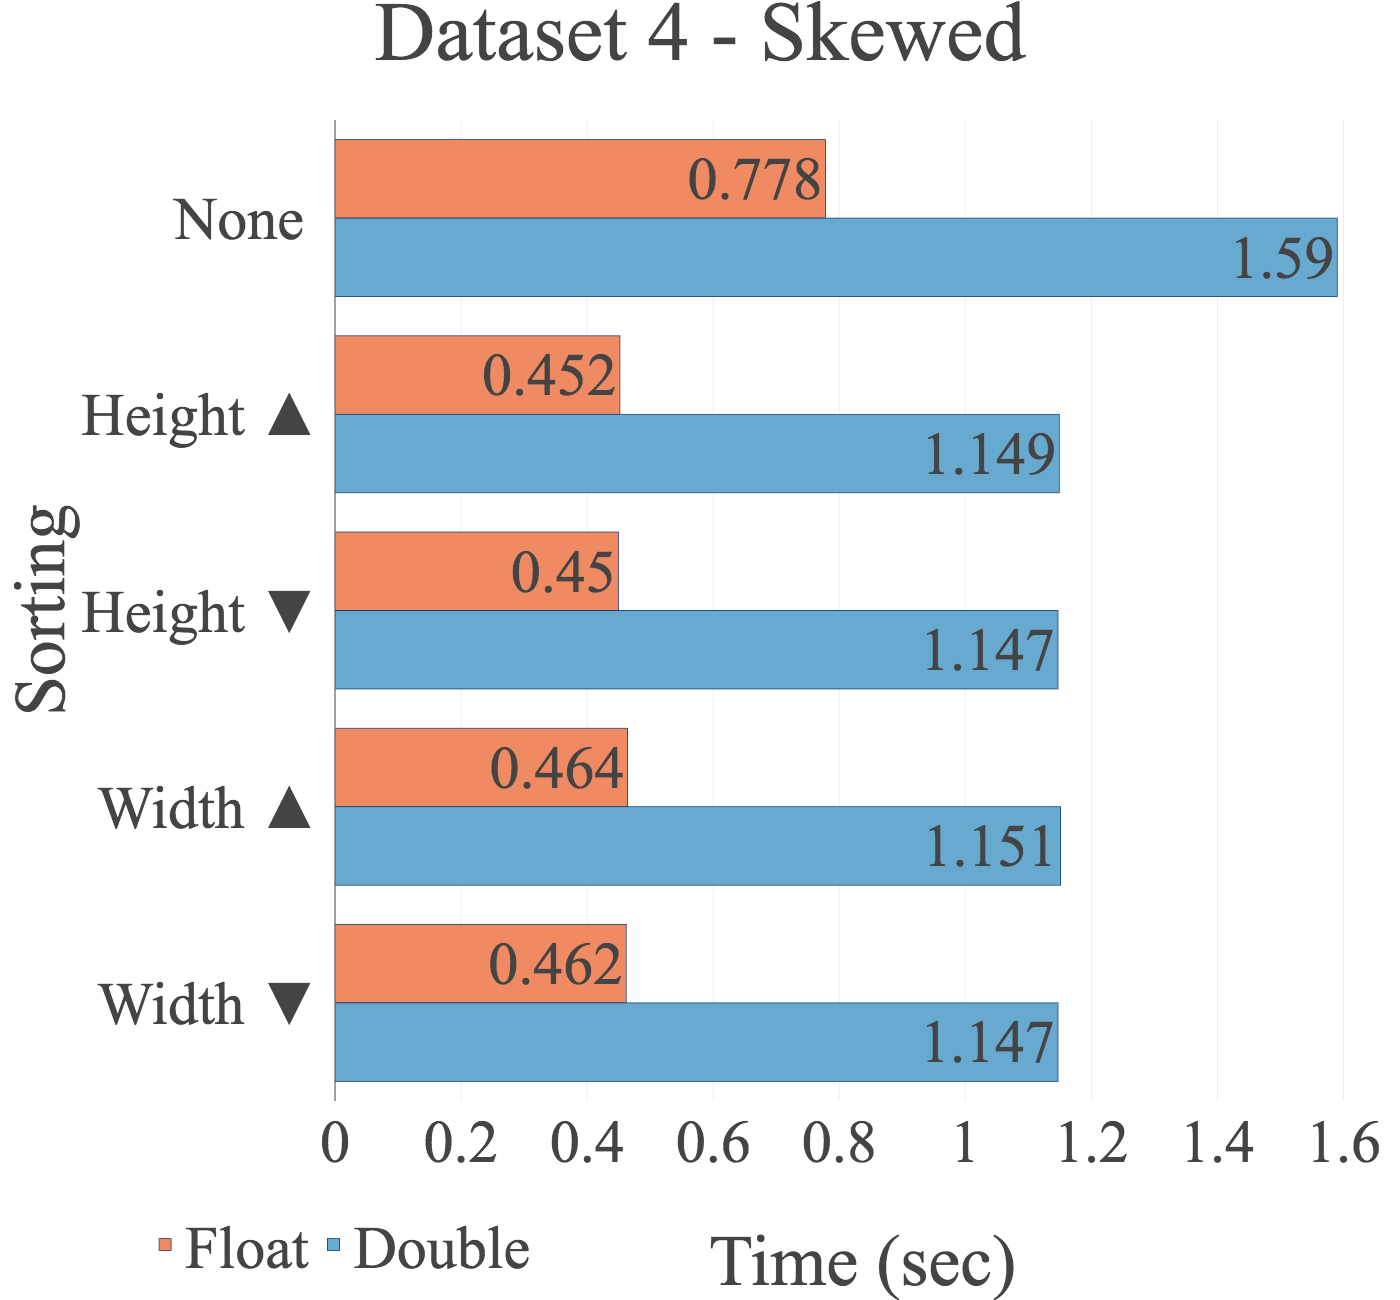
\includegraphics[width=1\textwidth]{img/experiments/multi-sorts-4_SKEWED.png}
\end{subfigure}
\begin{subfigure}{.62\textwidth}
  \centering
  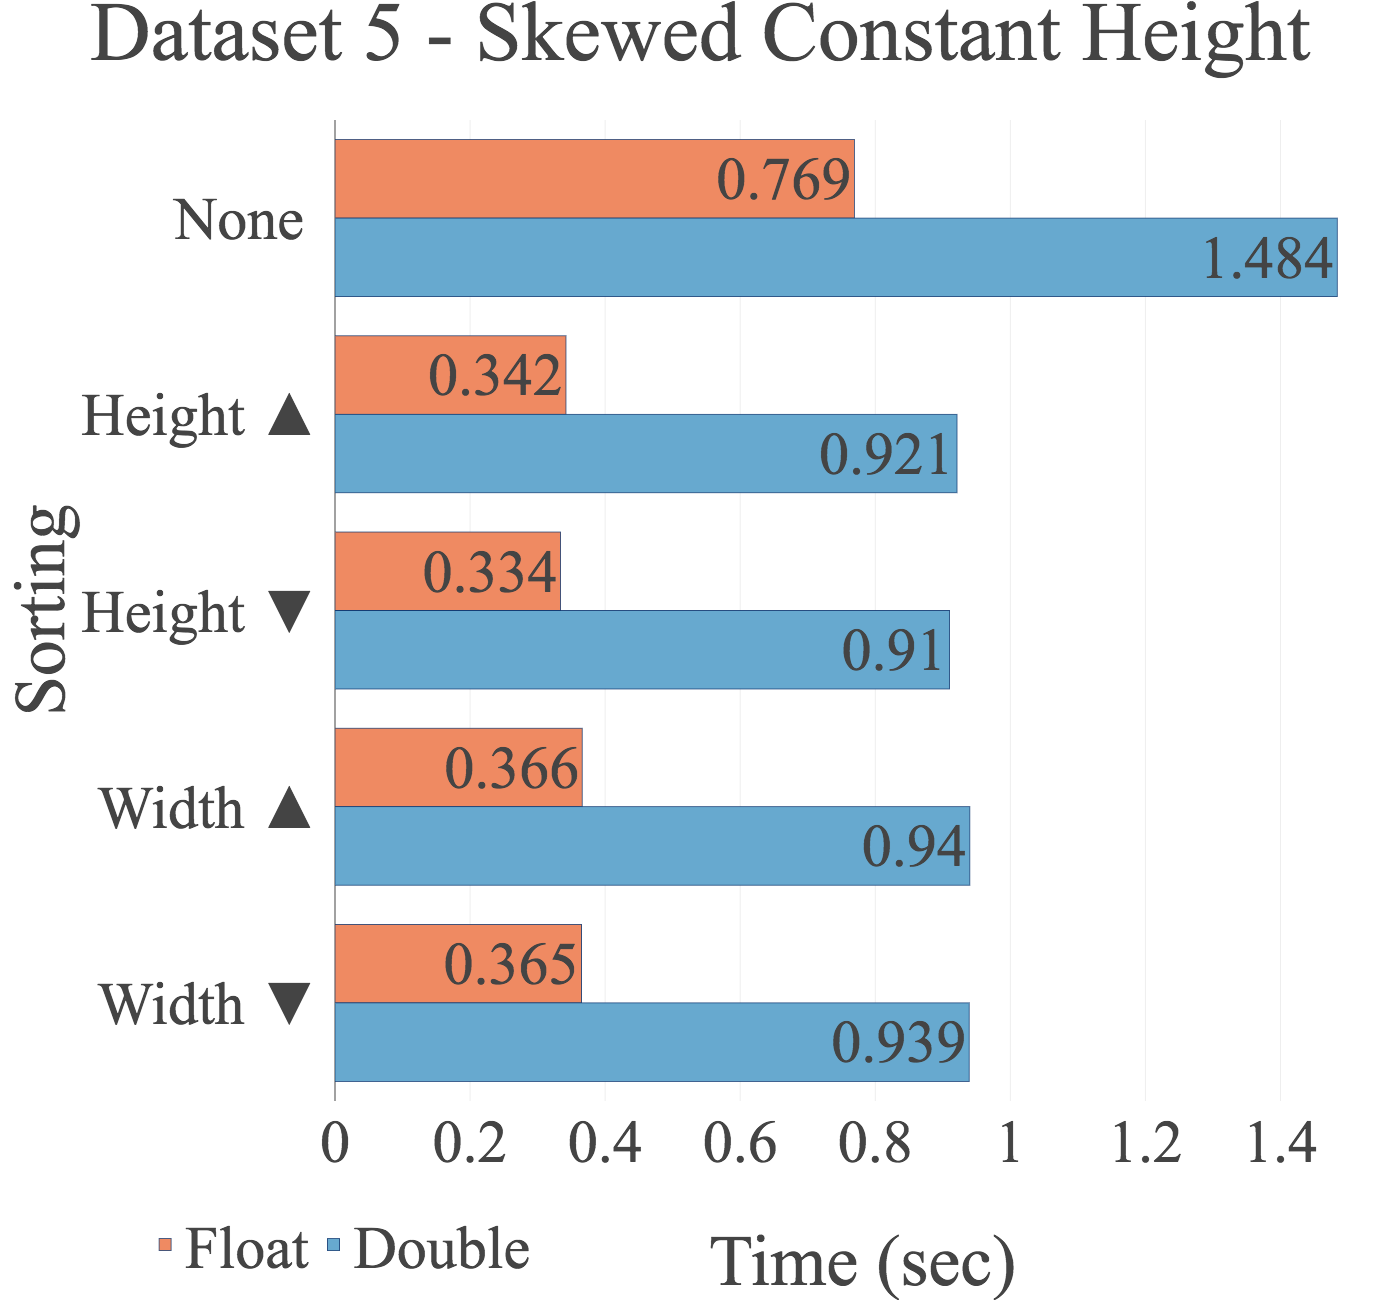
\includegraphics[width=1\textwidth]{img/experiments/multi-sorts-5_SKEWEDCONSTHEIGHT.png}
\end{subfigure}
\par\bigskip
\par\bigskip
\centering
\begin{subfigure}{.62\textwidth}
  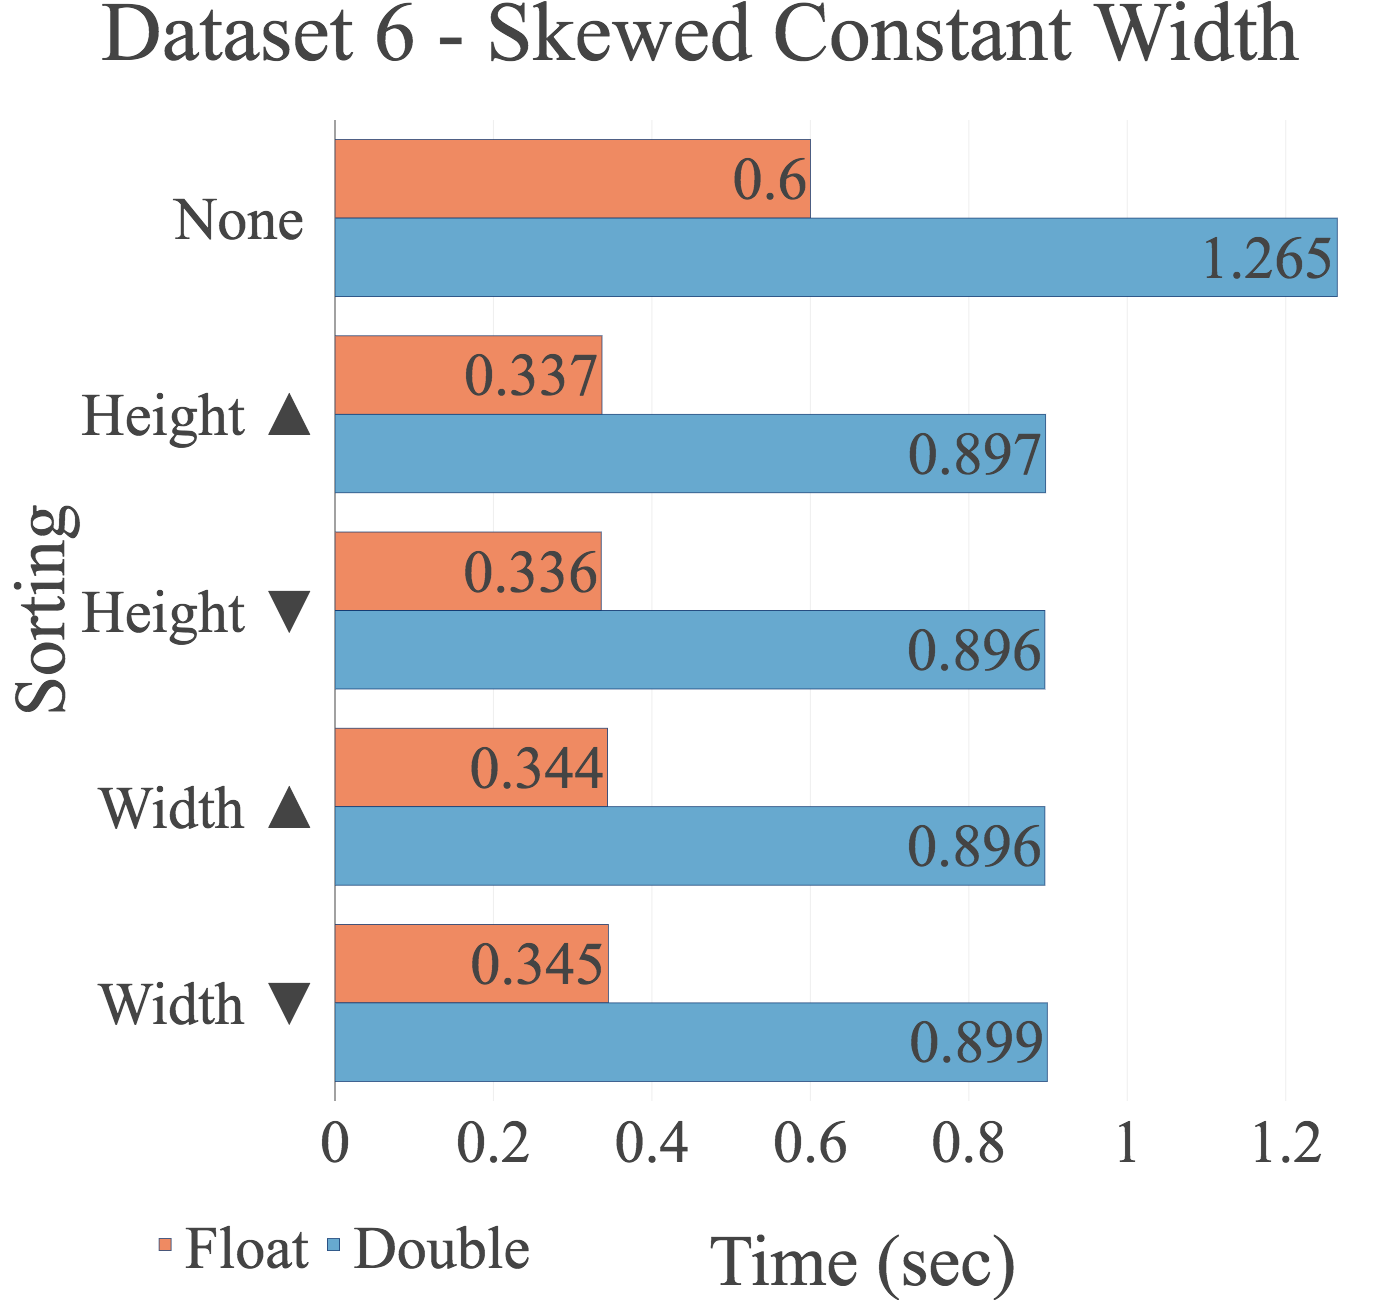
\includegraphics[width=1\textwidth]{img/experiments/multi-sorts-6_SKEWEDCONSTWIDTH.png}
\end{subfigure}
\end{adjustwidth}
\end{figure}

% SECTION END %

% SECTION START %
\section{Version Experiments (Average Memory)}
\begin{figure}[H]
\begin{adjustwidth}{-2cm}{-2cm}
\centering
\begin{subfigure}{.62\textwidth}
    \centering
    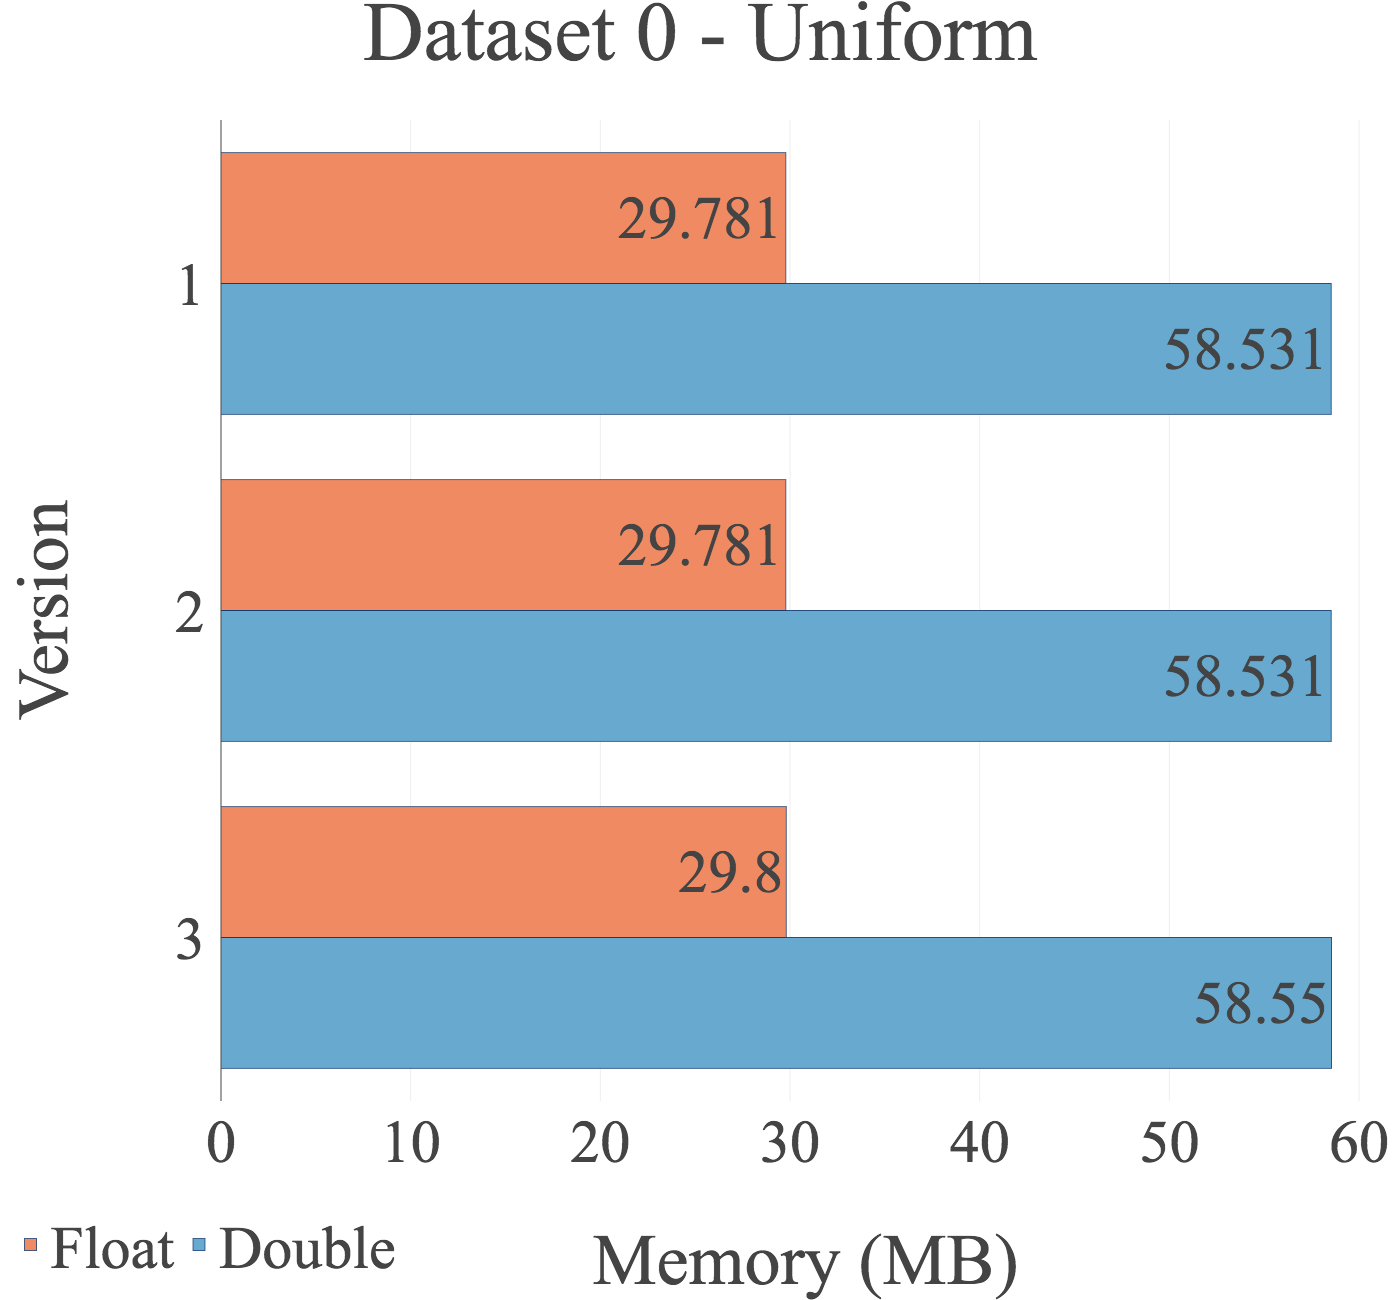
\includegraphics[width=1\textwidth]{img/experiments/mem-multi-versions-0_UNIFORM.png}
\end{subfigure}
\begin{subfigure}{.62\textwidth}
    \centering
    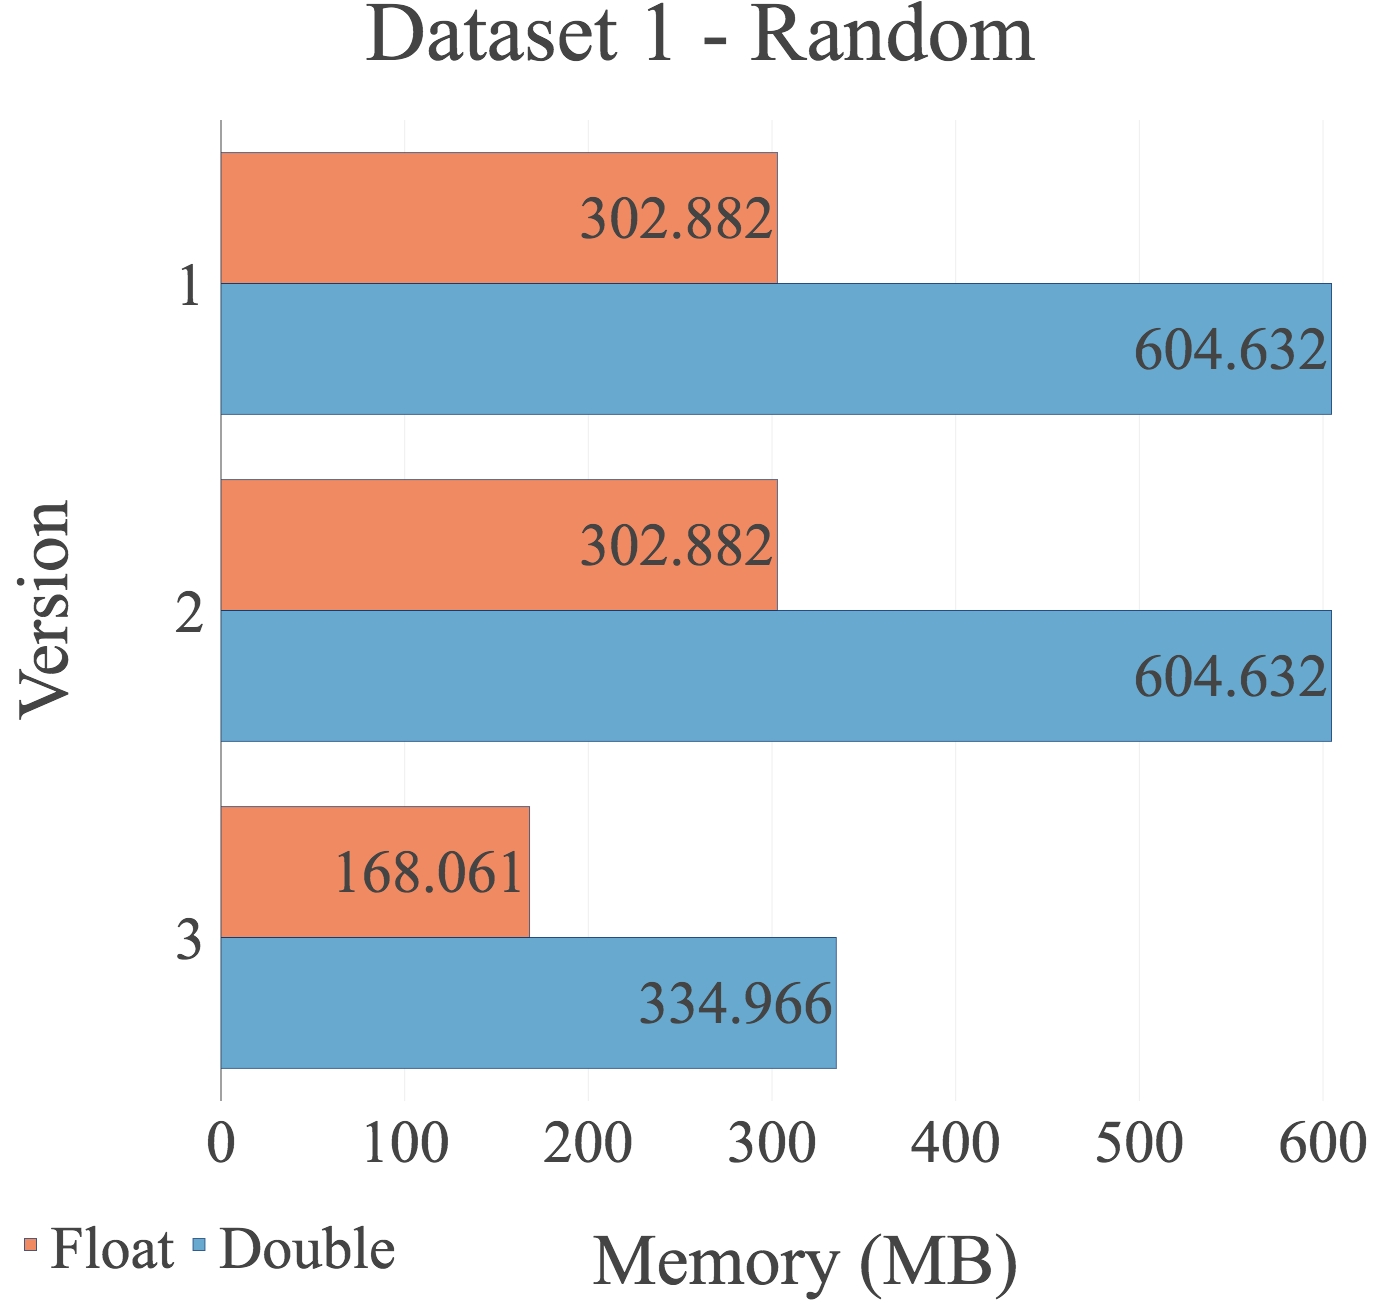
\includegraphics[width=1\textwidth]{img/experiments/mem-multi-versions-1_RAND.png}
\end{subfigure}
\par\bigskip
\par\bigskip
\begin{subfigure}{.62\textwidth}
  \centering
  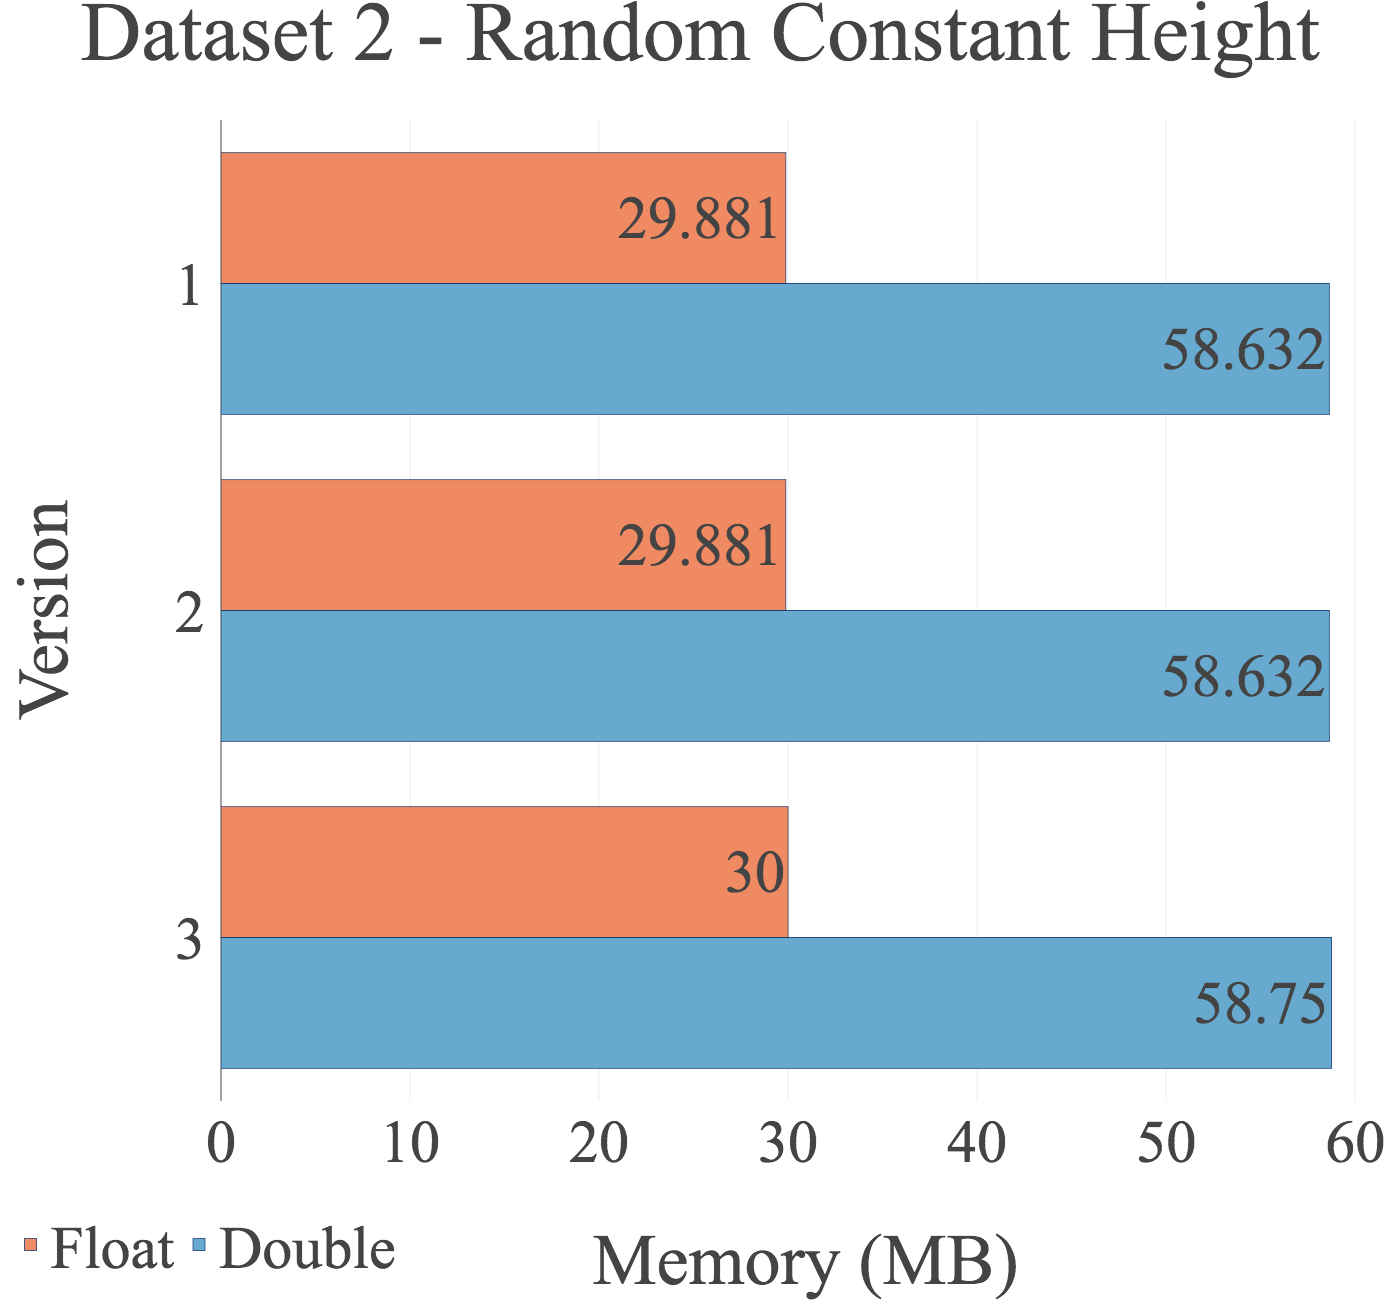
\includegraphics[width=1\textwidth]{img/experiments/mem-multi-versions-2_RANDCONSTHEIGHT.png}
\end{subfigure}
\begin{subfigure}{.62\textwidth}
  \centering
  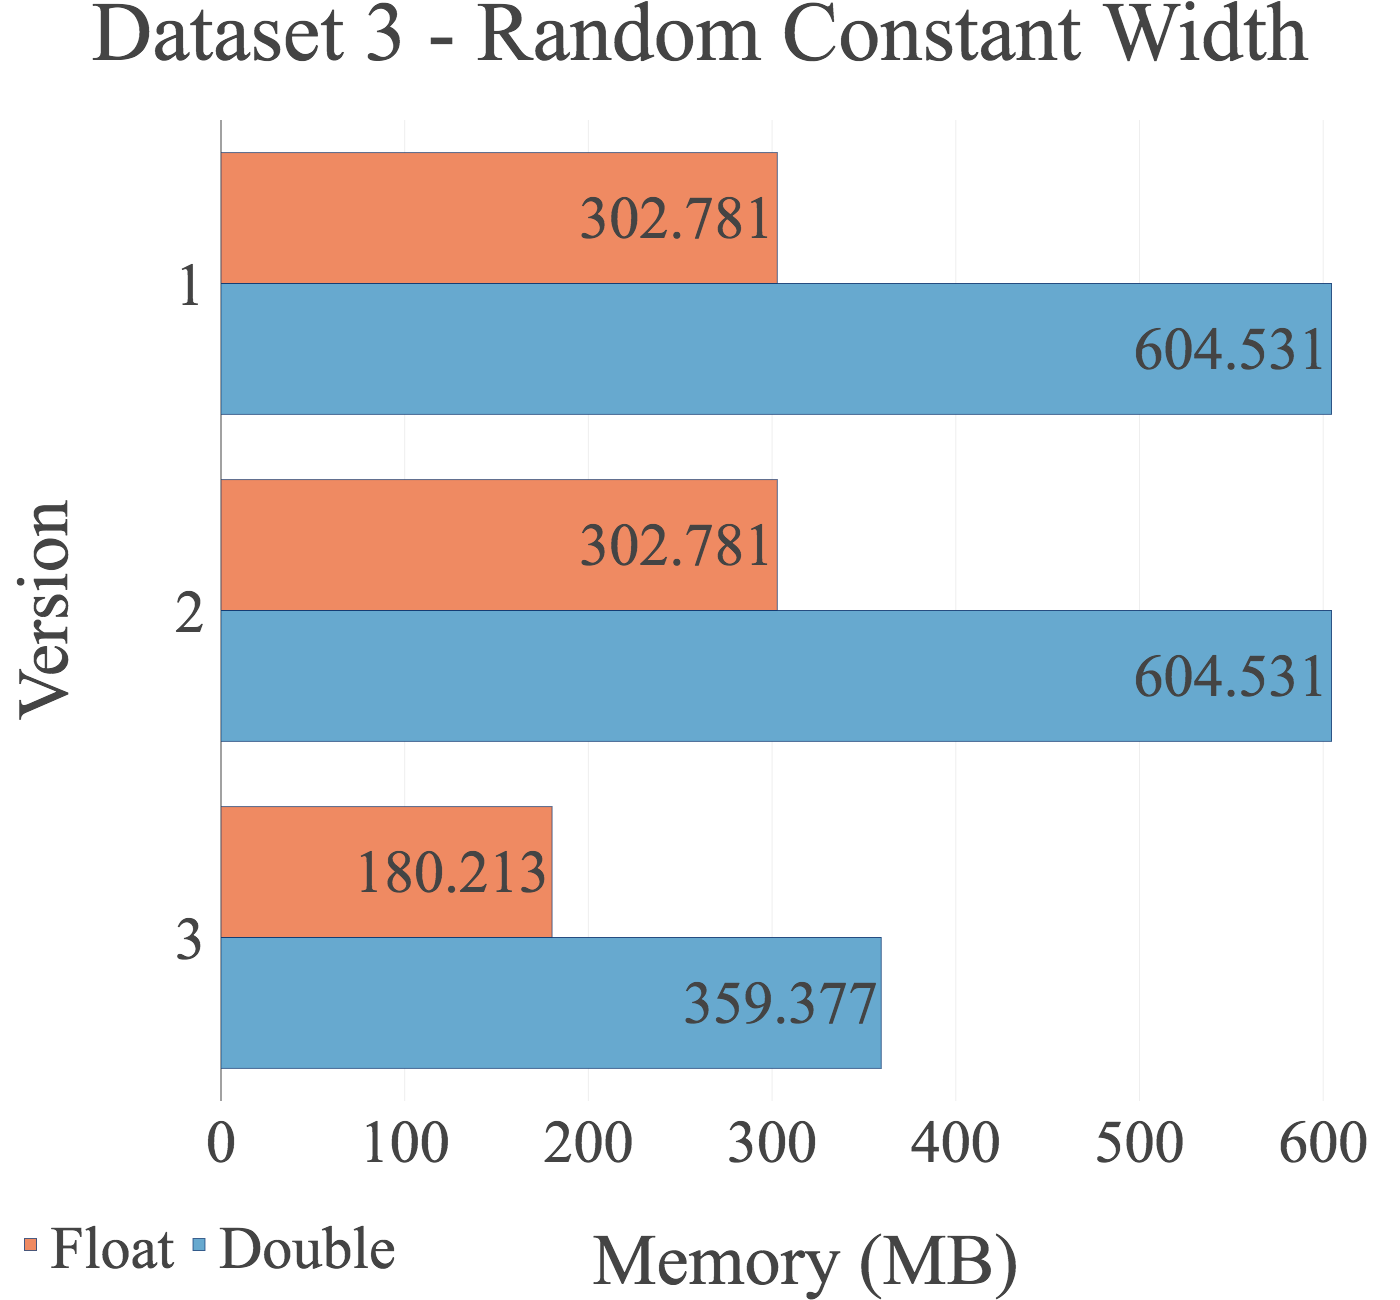
\includegraphics[width=1\textwidth]{img/experiments/mem-multi-versions-3_RANDCONSTWIDTH.png}
\end{subfigure}
\end{adjustwidth}
\end{figure}

\begin{figure}[H]
\begin{adjustwidth}{-2cm}{-2cm}
\begin{subfigure}{.62\textwidth}
  \centering
  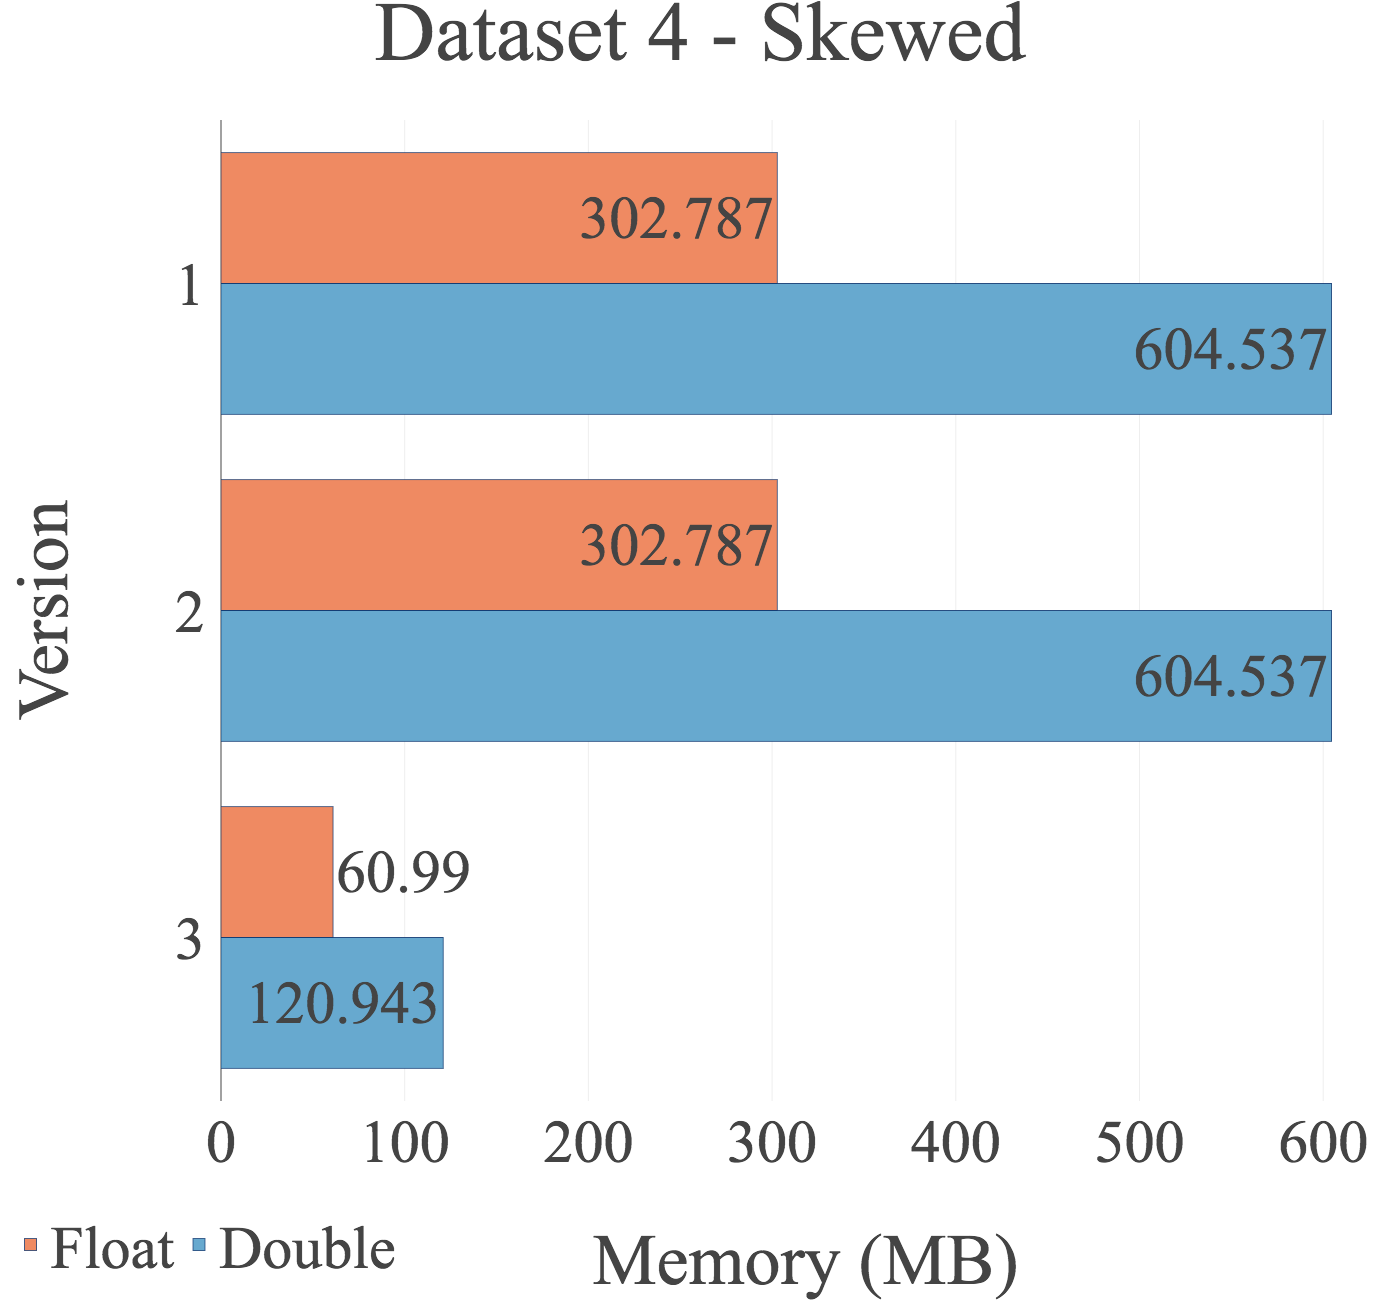
\includegraphics[width=1\textwidth]{img/experiments/mem-multi-versions-4_SKEWED.png}
\end{subfigure}
\begin{subfigure}{.62\textwidth}
  \centering
  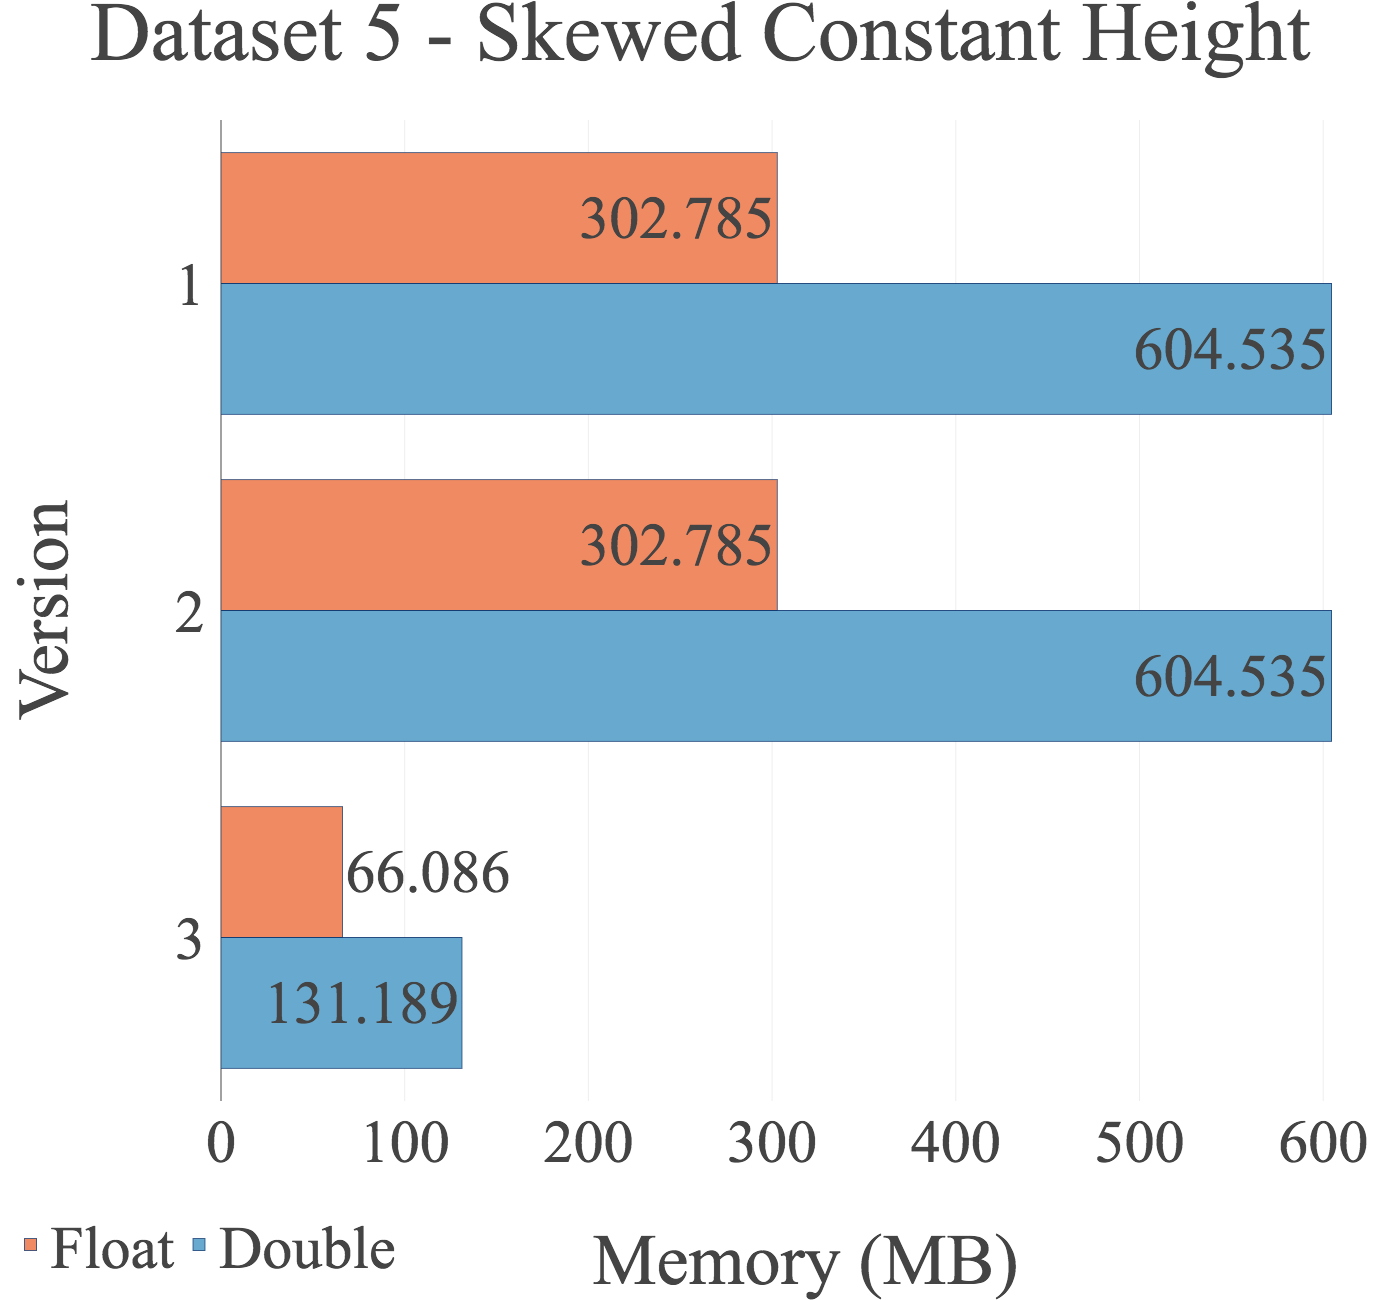
\includegraphics[width=1\textwidth]{img/experiments/mem-multi-versions-5_SKEWEDCONSTHEIGHT.png}
\end{subfigure}
\par\bigskip
\par\bigskip
\centering
\begin{subfigure}{.62\textwidth}
  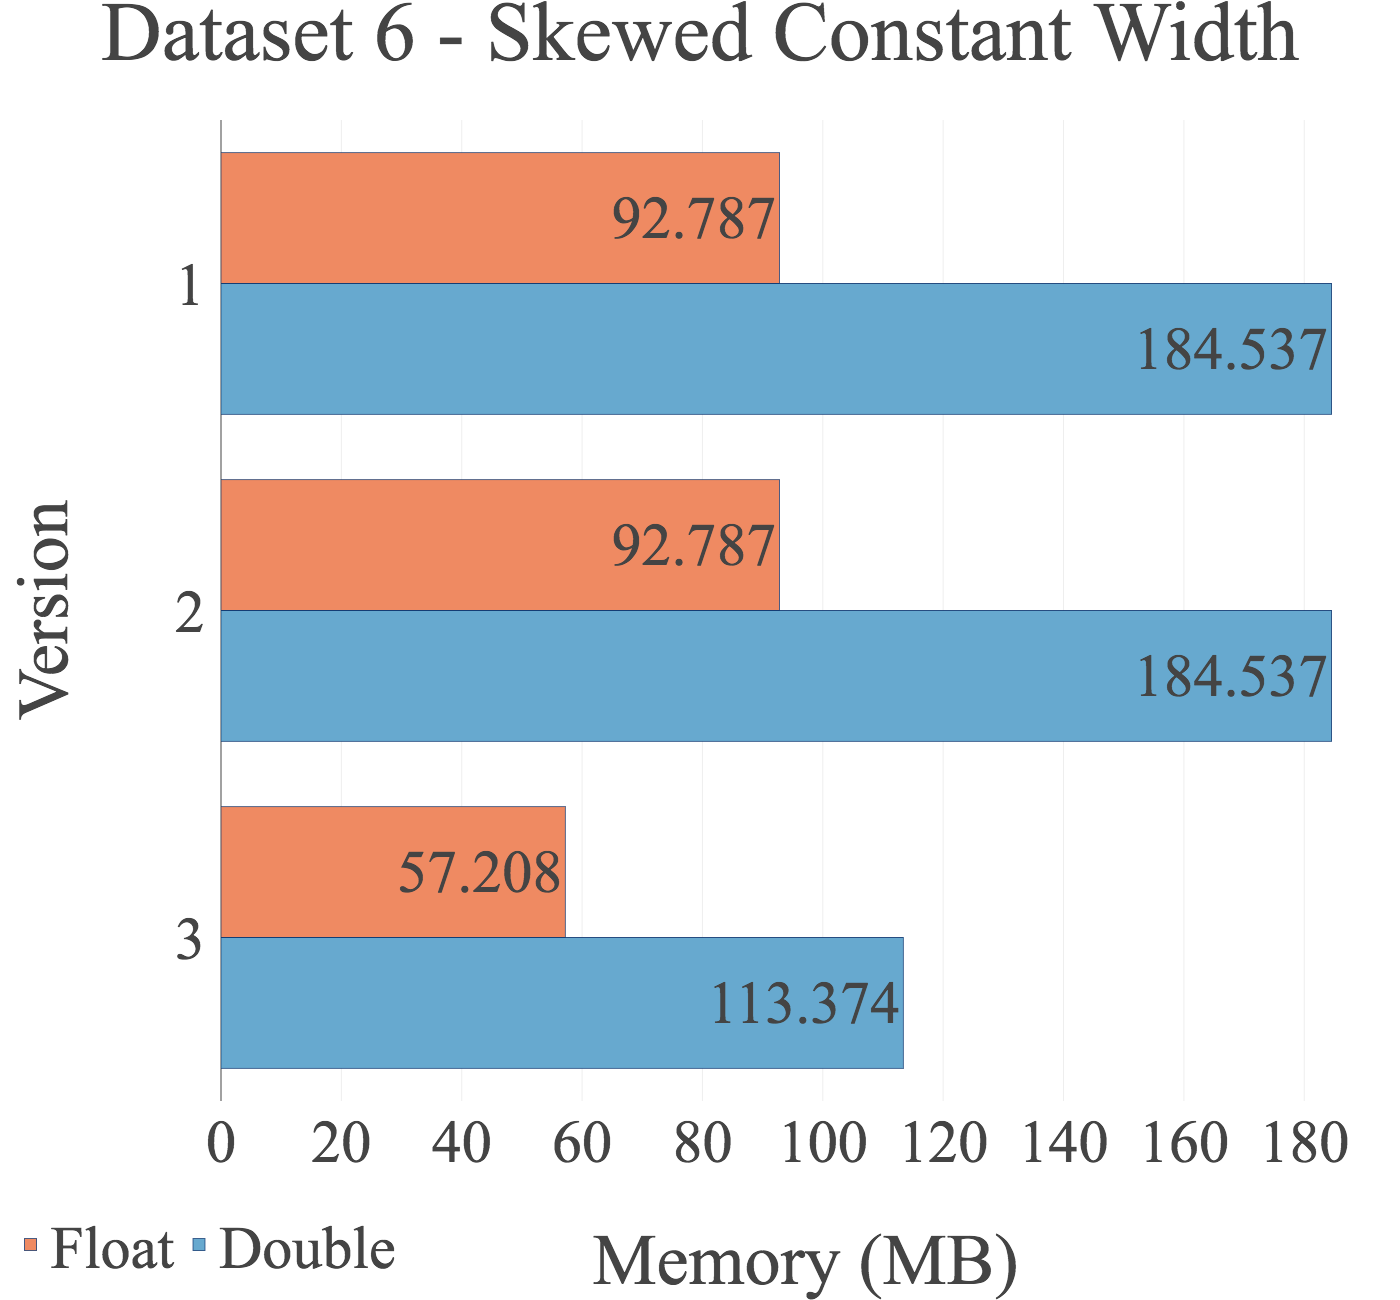
\includegraphics[width=1\textwidth]{img/experiments/mem-multi-versions-6_SKEWEDCONSTWIDTH.png}
\end{subfigure}
\end{adjustwidth}
\end{figure}

% SECTION END %
